\chapter{Desarrollo}

En este capítulo se describe el desarrollo del sistema en general: la selección de la técnica, el desarrollo de la técnica seleccionada y la selección del lenguaje de programación.

A continuación, en la \textbf{sección \ref{section:selecciontecnica}} se describe, a manera de resumen: las diferentes técnicas tomadas en cuenta durante la investigación y los porqués de la técnica seleccionada.

Después en la \textbf{sección \ref{section:desarrolloFIS}}, se describe el proceso de diseño del \textit{Sistema de Inferencia Difuso} bajo una metodología de mejora iterativa. El sistema tiene como objetivo calcular el tiempo de la fase en verde de un semáforo, que mediante la estructura propuesta y un preprocesamiento de los datos, permitirá gestionar diferentes tipos de intersecciones.

Posteriormente en la \textbf{sección \ref{section:desarrolloAlgoritmo}} se modela, mediante diagramas UML, la arquitectura del software desarrollado. El resultado es una micro-librería que permite \emph{expresar las variables y reglas del sistema difuso en notación de objetos}. Además, se modela la estructura propuesta para integrar la técnica seleccionada, a un sistema de control (a un algoritmo de sincronización) de semáforos y así, posibilitar la aplicación del sistema a una intersección con número no-estático de avenidas y fases.

\section{Preliminares}
Antes de continuar con el diseño del sistema, se considera adecuado aclarar algunos puntos acerca de:

\paragraph{El enfoque} presentado en este proyecto difiere con el resto en que, fue diseñado para ser embebido dentro de un algoritmo de sincronización de semáforos más general, de esta manera la tarea del \textit{FIS} se centra en determinar el tiempo en verde, dejando los detalles de sincronización en manos de un segundo algoritmo (también propuesto y desarrollado en este proyecto).

%El segundo algoritmo se encarga no solo del \emph{pre} y \emph{post} procesamiento de los datos de entrada y salida, sino que también define un marco de trabajo para la implementación final por parte del usuario final, valga la redundancia.

\paragraph{El pre-procesamiento} de los datos permite, mediante un proceso matemático sencillo, adaptar el \emph{FIS} propuesto a cruces con un número arbitrario de avenidas y fases, por ejemplo, intersecciones de: 2 avenidas y 2 fases, 4 avenidas y 2 fases o 4 avenidas y 4 fases. De esta manera se logra integrar una técnica de inteligencia artificial con un segundo algoritmo para la sincronización de semáforos.

%\paragraph{Lenguaje de programación}



\begin{wrapfigure}{r}{4cm}
	
\includegraphics[width=4cm]{Sources/logo_cpp11.jpg}
	%\captionof{figure}{C++ 11}
\end{wrapfigure}

\paragraph{La elección del lenguaje de programación} para la implementación del algoritmo fue bastante sencilla. Se requería un lenguaje eficiente que permitiera tener un control fino del proceso de inferencia, además de que permitiera que el algoritmo fuese portable entre plataformas. Por ello, se optó por el lenguaje de programación \emph{C++}, en específico, el estándar \emph{ISO C++11}.

C++ es uno de los más eficientes, con herramientas como punteros y referencias que evitan el desperdicio de memoria además de la \emph{semántica de movimiento} incluida en el estándar \textsc{C++11} que, aligera el paso de objetos de gran tamaño entre funciones (como los vectores usados en el proceso de inferencia). Por lo dicho anteriormente y por su amplia disponibilidad de compiladores en casi todas las plataformas, C++ resulta la elección perfecta para este proyecto.

\textbf{Paradigma} C++ es un lenguaje multiparadigma, permite trabajar usando programación estructurada, orientada a objetos e incluso funcional. En este proyecto se decidió hacer uso del paradigma orientado a objetos, debido a que se busca crear piezas de software altamente reutilizables y expresivas.

\section{Selección de la técnica}\label{section:selecciontecnica}
Después de investigar acerca de las principales ramas de la Inteligencia Artificial (véase sección \ref{cap:ramasdelaia}), se decidió optar por el uso de una técnica de Lógica Difusa; a saber, un \emph{Sistema Inferencia Difusa (FIS por sus siglas en inglés)}. Cabe mencionar que esta técnica está siendo ampliamente usada en la optimización del tráfico vehicular (véase la tabla \ref{table:estadodelarte}), esto se debe en parte, a que permite razonar sobre términos imprecisos como ``\emph{muchos carros}'' o ``\emph{poca congestión}''.

La elección de esta técnica sobre las otras se debe a varios factores: 

\paragraph{Algoritmos Genéticos} son una buena opción ya que podrían permitir probar diferentes asignaciones de tiempo, evaluar su desempeño y, así, ir depurando hasta encontrar la configuración optima de tiempos. Sin embargo, debido que la evaluación del desempeño podría ocasionar una congestión bastante alta, no es factible evaluarlo en un entorno real. Otra opción es evaluar el algoritmo en un entorno simulado, por desgracia, el tiempo requerido para la desarrollo del AG, del entorno de simulación y su correspondiente modelo matemático, va más allá del disponible para este proyecto.

\paragraph{Redes Neuronales Artificiales} estás son de gran ayuda en tareas como reconocimiento de voz, clasificación automática, tratamiento de imágenes entre otros. Sin embargo, desarrollar de una RNA para determinar el cambio de fase de un semáforo, podría llevar a lidiar con dificultades innecesarias, dificultades inherentes al entrenamiento de la propia red.

\paragraph{Sistemas Expertos} a primera vista puede parecer una buena idea, sin embargo, los problemas vienen al momento de expresar el conocimiento del experto en términos cuantitativos ya que no es muy fácil decidir en qué punto se le debe ceder el paso a una avenida u otra.

Una variante, son los sistemas difusos. Aquí sucede algo importante: los controladores difusos y los sistemas expertos difusos son en esencia lo mismo: Sistema de Inferencia Difusa. Es decir, ambos se basan en la inferencia difusa, por ejemplo: la inferencia de mamdani.

\paragraph{Sistema de Inferencia Difusa} la gran ventaja de estos sistemas es que, gracias a que usan lógica difusa, permiten expresar el conocimiento (reglas) en términos coloquiales que poseen cierto grado de incertidumbre. Así, es posible modelar un sistema que de preferencia a las avenidas con muchos carros y, definir el término muchos carros con una función de membresía centrada en 7. De esta manera, entre más cercano sea a 7 el valor evaluado, mayor peso tendrá en la decisión tomada por el sistema.

Estos sistemas permiten lidiar con la información que no es tan precisa o, en el caso de este proyecto, permite razonar sobre términos como muchos carros o poca congestión. Términos para los cuales, no es fácil asignar un intervalo de valores. Es por eso que se decidió usar un Sistema de Inferencia Difusa para dotar de cierto grado de \textit{``inteligencia''} a un algoritmo de control de semáforos.

\section{Diseño del Sistema de Inferencia}\label{section:desarrolloFIS}
En esta sección se expone de manera metodológica las diferentes configuraciones, resultados y conclusiones que se obtuvieron en el desarrollo del sistema. Para la configuración se sigue una estrategia de mejora iterativa hasta alcanzar el resultado deseado.

\subsection{Configuraciones aplicadas de manera general}

\textbf{Selección de operadores}\\ 
Debido a la variedad de operadores que pueden ser usados en la inferencia difusa, a continuación se muestran los operadores usados en este proyecto.

\begin{multicols}{2}
\begin{itemize}
	\item \textbf{Método AND:} operador mínimo \emph{min}.
	\item \textbf{Método OR:} operador máximo \emph{max}.
	\item \textbf{Implicación:} operador mínimo \emph{min}.
	\item \textbf{Agregación:} operador máximo \emph{max}.
	\item \textbf{Defuzzificación:} centroide \emph{$\frac{\sum \mu(x).x}{\sum \mu(x)}$}.
\end{itemize}
\end{multicols}
\subsubsection{Selección de variables}
Como se mencionó, el diseño del sistema difuso, se enfoca en el cálculo de tiempos óptimos para las fases verdes de los semáforos, para ello, se consideran tres aspectos, a saber: la cantidad de autos a los que se les cederá el paso, la cantidad de autos que quedarán en espera y, el número de carriles por avenida. Estos datos permitirán al sistema de inferencia dar preferencia a aquellas avenidas con un mayor número de carriles y/o mayor número de autos.

La selección de variables de entrada y salida del sistema, debe ser cuidadosa para no elevar la complejidad del sistema ni caer en redundancias. En el desarrollo de este sistema se ha seguido la filosofía KISS\footnote{Keep it simple, Stupid!} que plantea el desarrollo de sistemas sencillos, flexibles y escalables.

Al seleccionar las variables hay que cuidar que estás estén correlacionadas con las variables de salida, además, se debe mantener el número de variables y particiones al mínimo necesario.

Habiendo dicho lo anterior, se presenta la selección de variables, así, como una breve justificación de su elección. \\

\textbf{Variables de entrada}\\
\textit{a) Vehículos} La variable vehículos indica la cantidad de autos que se encuentran en la avenida a la que se le dará el paso\\
\textit{b) Congestión} La variable congestión se propone como un indicador que sume de manera ponderada la cantidad de automóviles y carriles. A saber, la suma ponderada se define como:

\begin{displaymath}
\frac{\sum_{i=1}^{n} x_i * w_i}{\sum_{i=1}^{n} w_i}
\end{displaymath}
Donde:

{\setlength{\baselineskip}{0.7\baselineskip}\begin{description}
	\item $x$ es un vector con la cantidad de autos de las avenidas.
	\item $w$ es un vector de pesos que describe la prioridad de cada avenida.
\end{description}}

Además, se propone el cálculo de los pesos de las avenidas como una función directamente proporcional al número de carriles de la avenida en cuestión e inversamente proporcional al número total de carriles , i,e:

\begin{displaymath}
w_i = \frac{ c_i }{\sum_{j=1}^{j=n} c_j}
\end{displaymath}
Donde:
{\setlength{\baselineskip}{0.7\baselineskip}\begin{description}
		\item $C$ es un vector con la cantidad de carriles de cada avenida.
		\item $i$ es la avenida a evaluar.
\end{description}}
De esta manera el sistema resulta lo suficientemente flexible para ser aplicado a intersecciones de 2, 4, 8 o cualquier numero $n$ de avenidas (siempre y cuando tenga sentido).\\

\textbf{Variables de salida}\\
\textit{a) Tiempo} Con el fin de hacer el sistema fácilmente escalable, se propone como variable de salida la cantidad de segundos de la fase verde del semáforo en cuestión. Esto permitirá integrar el sistema de inferencia dentro de un algoritmo clásico de control de semáforos. Así, la \textit{inteligencia} se encuentra en la optima asignación de tiempos.

\newpage
\subsection{Configuración A}
La configuración presentada a continuación mantiene al mínimo el número de términos dentro de las variables de entrada y salida. 

\paragraph{Variable de entrada Vehículos} referente a la cantidad de vehículos en la avenida a la cual se le asignará la fase verde. La variable se encuentra definida en un universo de discurso $U = [0,12]$.

\begin{table}[!h]
	\centering
	\begin{tabular}{llr} \toprule
		Termino lingüístico & Función de membresía & Parámetros \\ \midrule
		Pocos & Triangular & [0, 0, 12 ] \\
		Muchos & Triangular & [0, 12, 12] \\ \bottomrule
	\end{tabular}
	\caption{Variable lingüística \textit{Vehículos}}
\end{table}


\paragraph{Variable de entrada Congestión} se refiere al índice ponderado de la cantidad de vehículos en las avenidas que quedaran a la espera durante la fase verde actual. La variable se encuentra definida en un universo de discurso $U = [0,12]$.

\begin{table}[!h]
	\centering
	\begin{tabular}{llr} \toprule
		Termino lingüístico & Función de membresía & Parámetros \\ \midrule
		Baja & Triangular & [0, 0, 12 ] \\
		Alta & Triangular & [0, 12, 12] \\ \bottomrule
	\end{tabular}
	\caption{Variable lingüística \textit{Congestión}}
\end{table}

\begin{figure}[H]
	\centering
	\subfigure[Variable lingüística Vehículos]{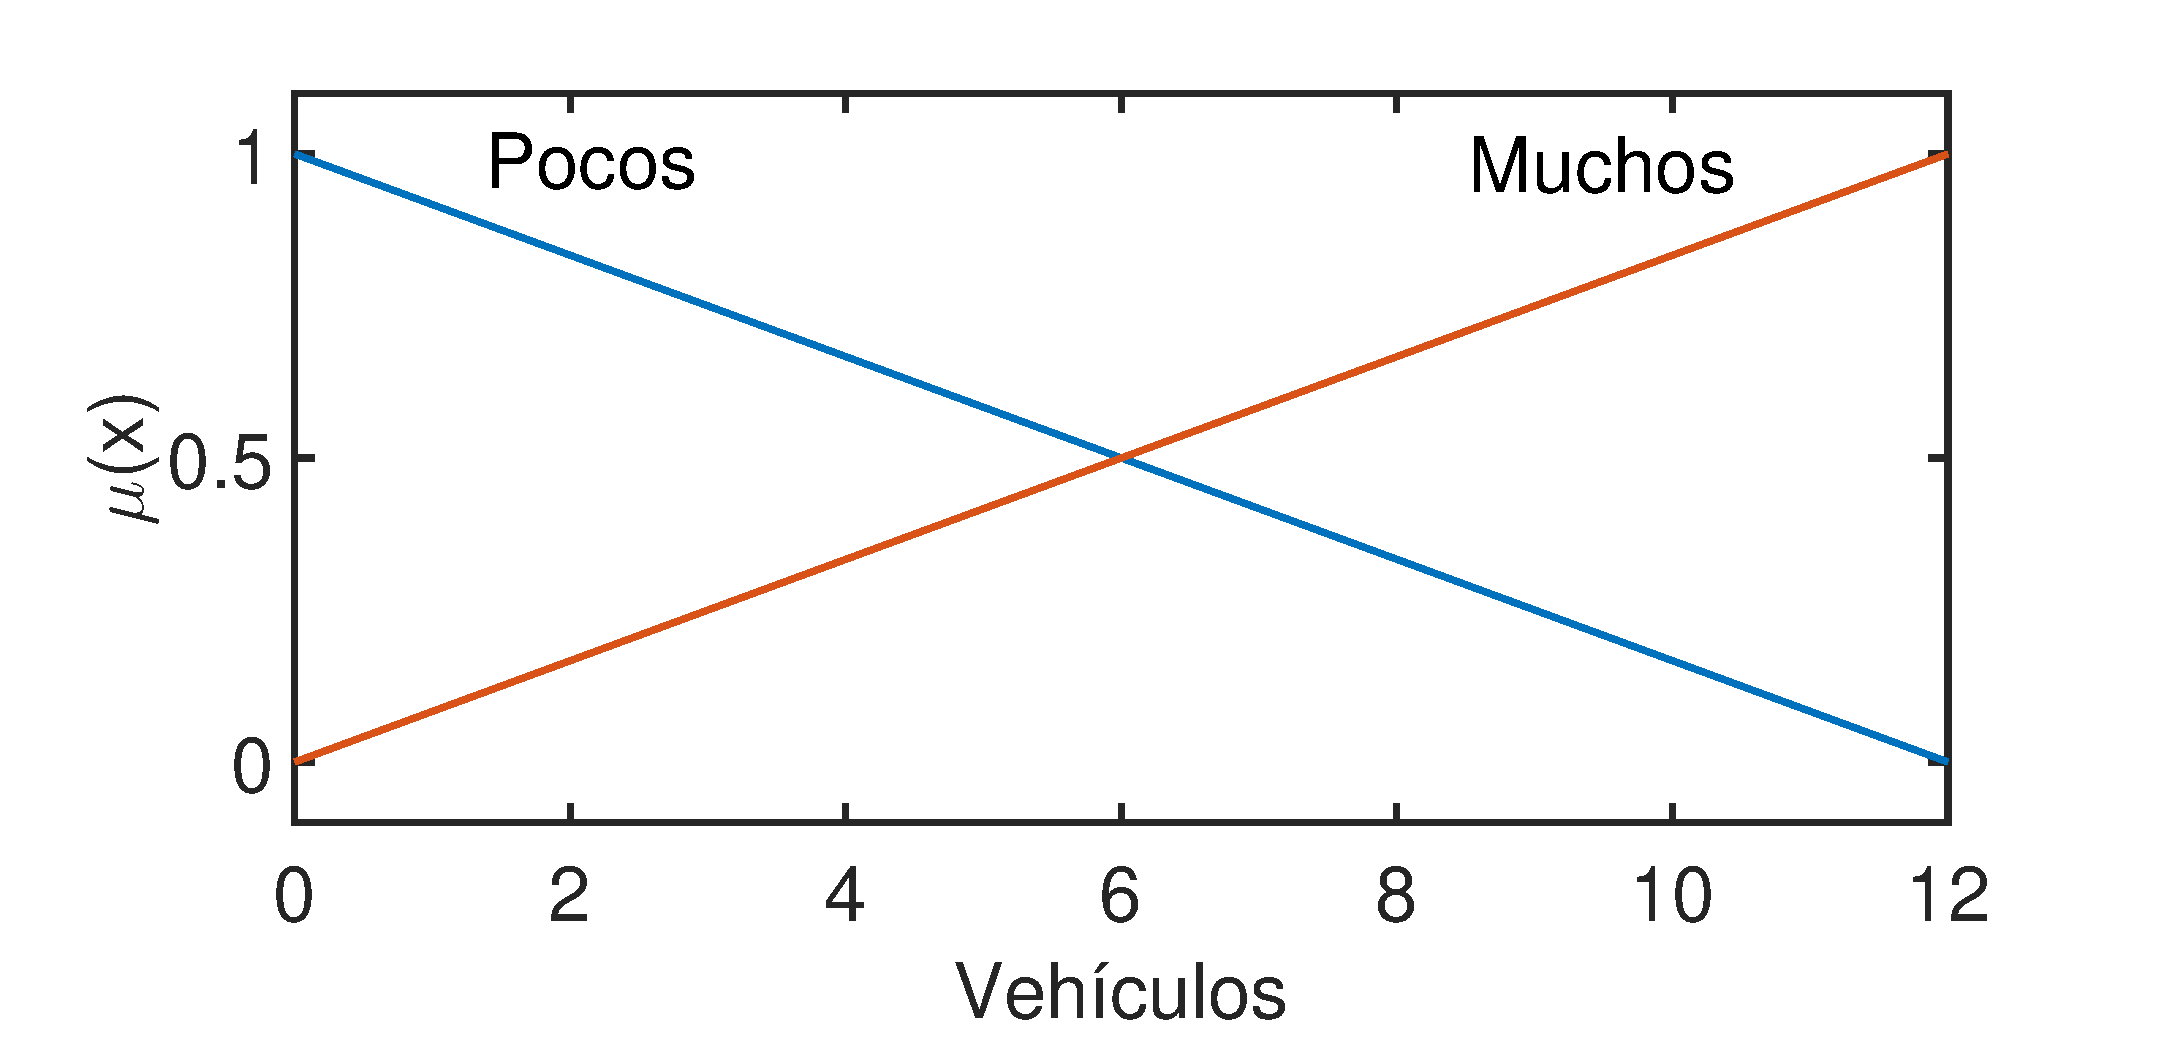
\includegraphics[height=4cm, width=8.1cm]{Variables/ConfigA_input1.eps}}
	\subfigure[Variable lingüística Congestión]{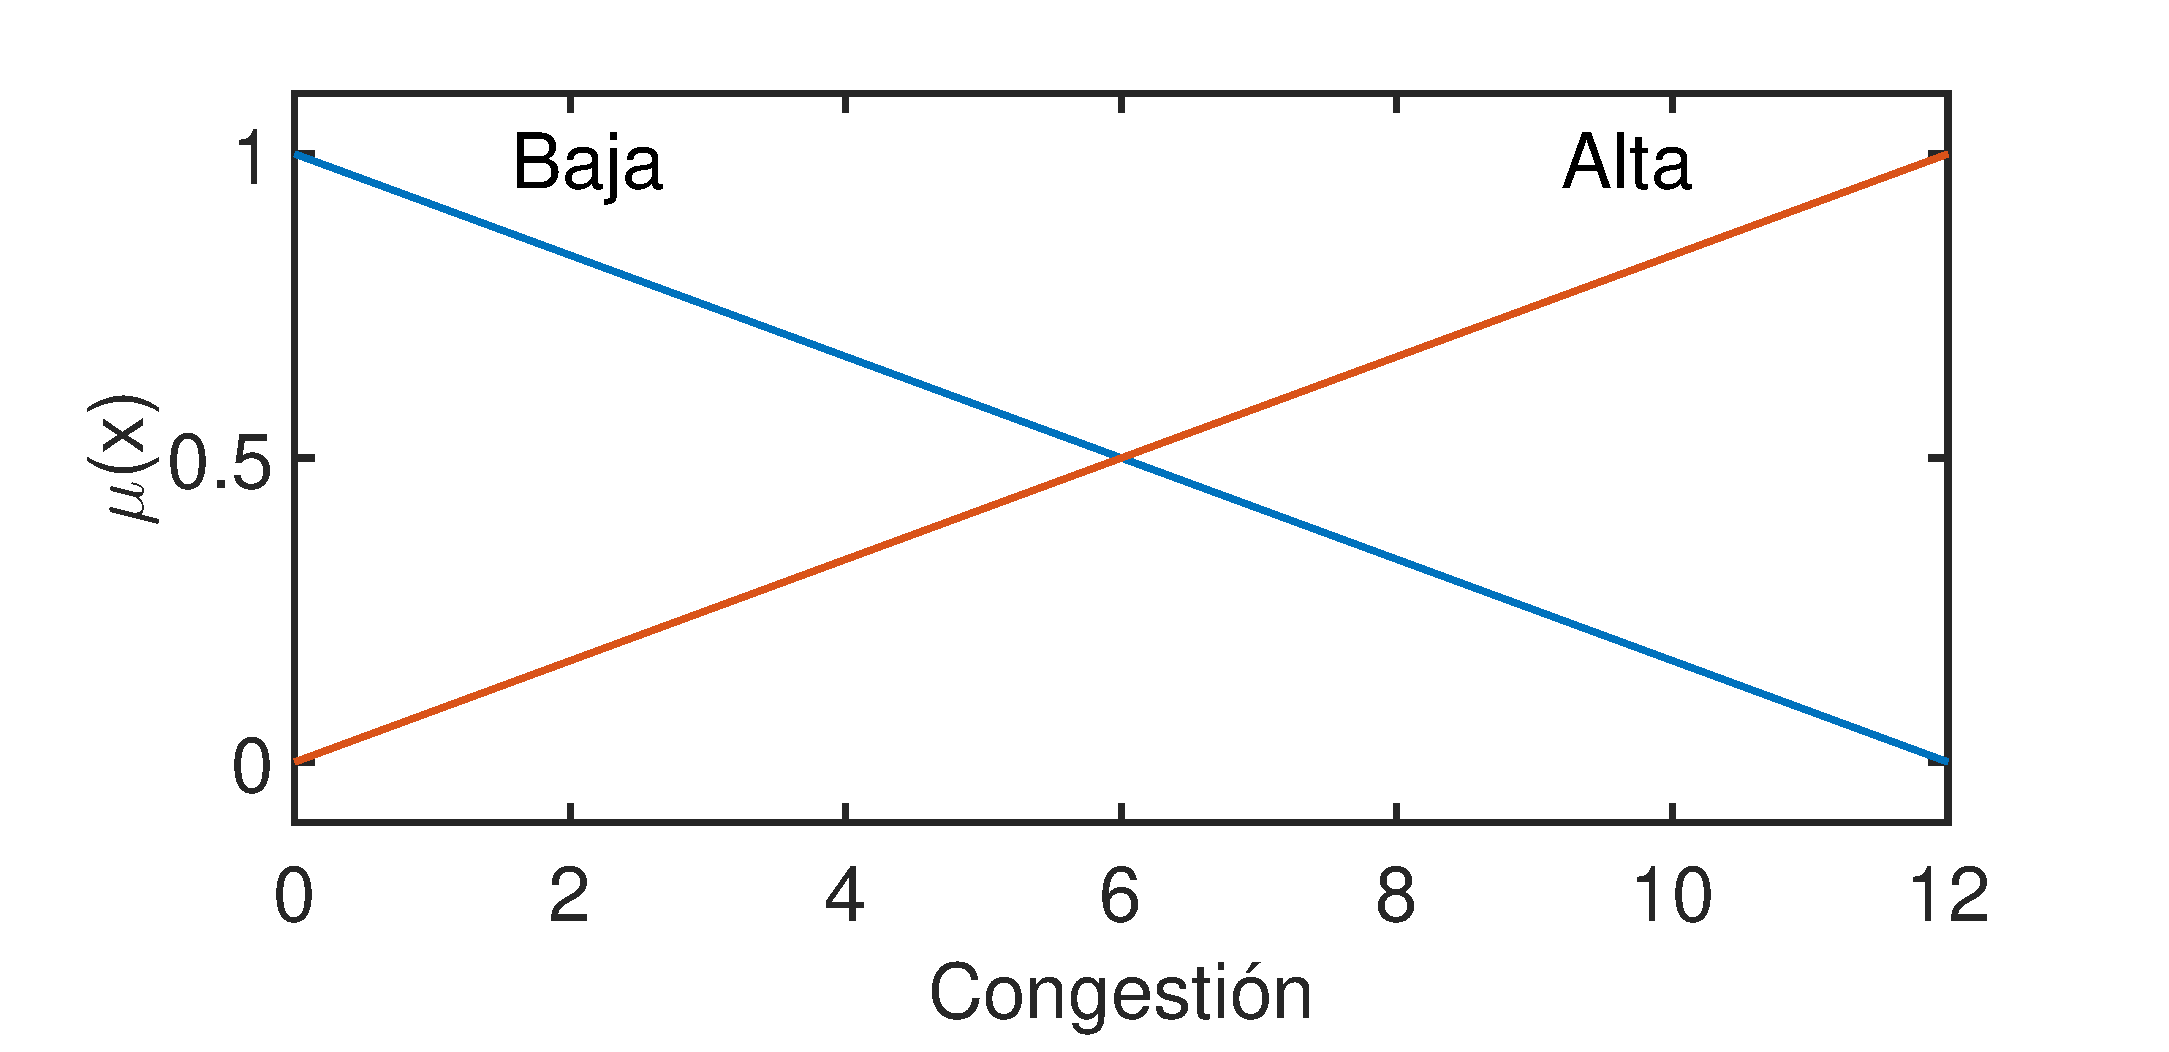
\includegraphics[height=4cm, width=8.1cm]{Variables/ConfigA_input2.eps}}
	\caption[Gráficas de las variables lingüísticas vehículos y congestión]{Representación gráfica de las variables lingüísticas Vehículos y Congestión }
\end{figure}

\newpage
\paragraph{Variable de salida Tiempo} se refiere al tiempo en segundos que le será asignada a la fase verde actual. La variable se encuentra definida en un universo de discurso $U = [0,90]$.

\begin{table}[!h]
	\centering
	\begin{tabular}{llr} \toprule
		Termino lingüístico & Función de membresía & Parámetros \\ \midrule
		Bajo & Triangular & [0, 0, 30 ] \\
		Medio & Triangular & [0, 30, 60] \\
		Moderado & Triangular & [30, 60, 90] \\
		Alto & Triangular & [60, 90, 90] \\ \bottomrule
	\end{tabular}
	\caption{Variable lingüística \textit{Tiempo}}
\end{table}

\begin{figure}[H]
	\centering
	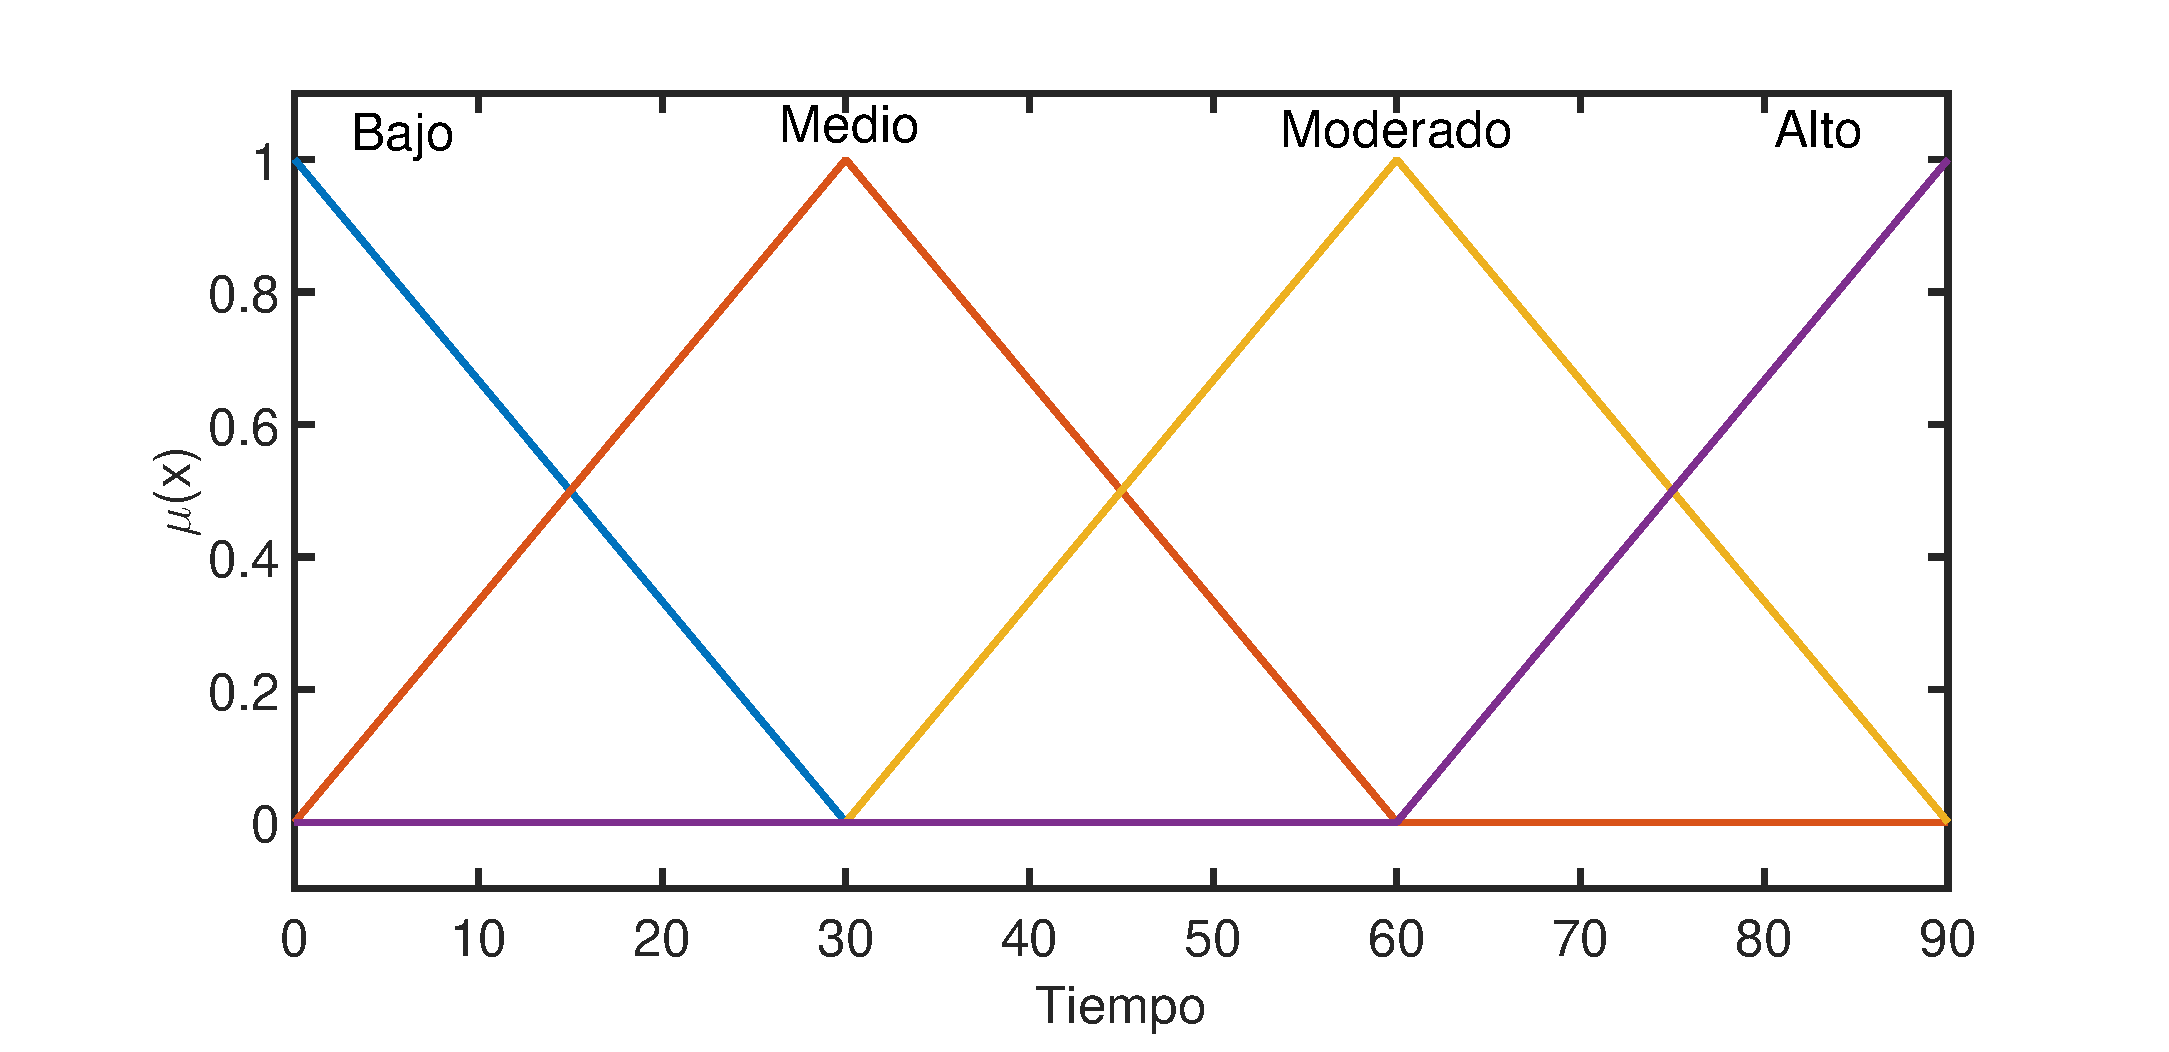
\includegraphics[height=5cm, width=12cm]{Variables/ConfigA_output1.eps}
	\caption[Gráfica variable lingüística tiempo - A]{Representación gráfica de la variable lingüística Tiempo}
\end{figure}

\subsubsection{Base de conocimientos}
La siguiente tabla muestra las reglas difusas empleadas en esta configuración.
\begin{longtable}[c]{lclcl} \toprule
	\multicolumn{3}{c}{Antecedente} & & Consecuente \\ \midrule
	Vehículos Pocos & Y & Congestión Baja& $\rightarrow$ & Verde Medio \\
	Vehículos Pocos & Y & Congestión Alta& $\rightarrow$ & Verde Bajo \\
	Vehículos Muchos &Y& Congestión Baja& $\rightarrow$ & Verde Alto \\
	Vehículos Muchos &Y& Congestión Alta& $\rightarrow$ & Verde Moderado \\ \hline
	\caption{Reglas difusas para la configuración \textit{A}}
\end{longtable}

\newpage
\subsubsection{Resultados}


Una vez diseñado e implementado el sistema de inferencia, se le suministraron valores de prueba para evaluar su desempeño. Los resultados de dicha evaluación se reflejan en la tabla siguiente:

\begin{table}[H]
	\centering
	\begin{tabular}{cccccc} \toprule
		$V \backslash C$ &  0 & 3 & 6 & 9 & 12 \\ \midrule
		0 & 30.00 & 28.99 & 26.21 & 20.86 & 09.70 \\
		3 & 39.02 & 39.03 & 37.69 & 35.58 & 33.96 \\
		6 & 46.40 & 45.83 & 45.00 & 44.16 & 43.59 \\
		9 & 56.03 & 54.41 & 52.30 & 50.96 & 50.97 \\
		12& 80.29 & 69.13 & 63.79 & 61.00 & 59.99 \\
		%\caption{Resultados de la evaluación para la configuración \textit{A}}
	\end{tabular}
	\caption{Resultados de la evaluación para la configuración}
\end{table}
Donde: la columna V son los valores de prueba de la variable Vehículos, la fila C son los valores de  prueba de la variable Congestión y las celdas son los tiempos (en segundos).




\subsubsection{Observaciones}
\begin{multicols}{2}

Después de evaluar el desempeño de la primera configuración se observa como efectivamente el tiempo asignado varía de acuerdo a las variables de entrada; sin embargo, el tiempo asignado para las entradas Vehículos = 0 y Congestión = 6, resulta excesivo puesto que la cantidad de vehículos a los que se les cederá el paso es mínimo (0) mientras que el índice de vehículos (6) que se mantendrán a la espera es bastante considerable.

\begin{figure}[H]
	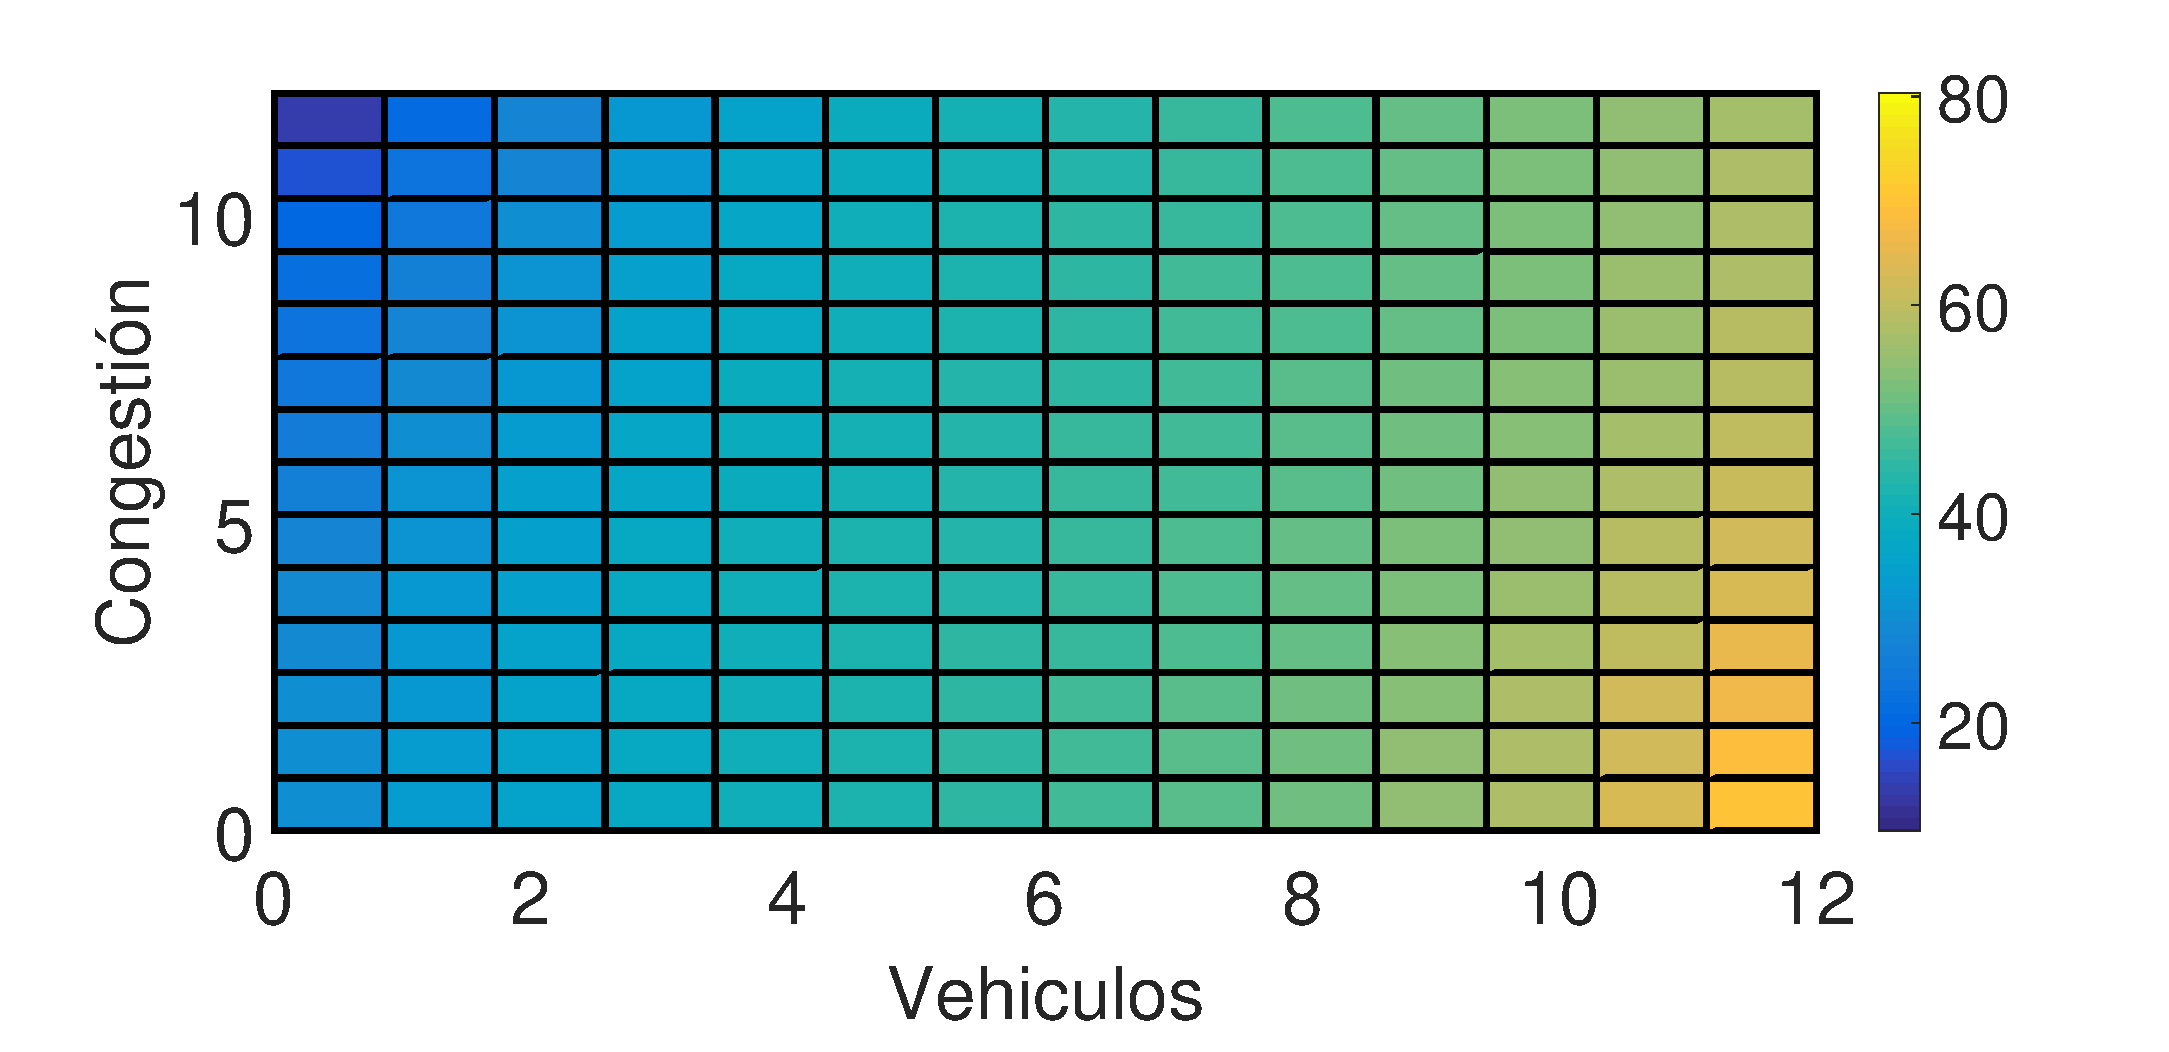
\includegraphics[width=0.5\textwidth]{Surfaces/Surface2D_A.eps}
	\caption{Superficie de control}
\end{figure}

\end{multicols}

 


\pagebreak
\subsection{Configuración B}
La configuración presentada en esta sección, ajusta los parámetros de las funciones de membresía de la variable de salida Tiempo. La configuración pasa a ser la siguiente: 

\paragraph{Variable de entrada Vehículos} Se mantiene sin cambios.

\begin{table}[!h]
	\centering
	\begin{tabular}{llr} \toprule
		Termino lingüístico & Función de membresía & Parámetros \\ \midrule
		Pocos & Triangular & [0, 0, 12 ] \\
		Muchos & Triangular & [0, 12, 12] \\ \bottomrule
	\end{tabular}
	\caption{Variable lingüística \textit{Vehículos}}
\end{table}


\paragraph{Variable de entrada Congestión} se mantiene sin cambios desde la configuración anterior.


\begin{table}[!h]
	\centering
	\begin{tabular}{llr} \toprule
		Termino lingüístico & Función de membresía & Parámetros \\ \midrule
		Baja & Triangular & [0, 0, 12 ] \\
		Alta & Triangular & [0, 12, 12] \\ \bottomrule
	\end{tabular}
	\caption{Variable lingüística \textit{Congestión}}
\end{table}

\begin{figure}[H]
	\centering
	\subfigure[Variable lingüística Vehículos]{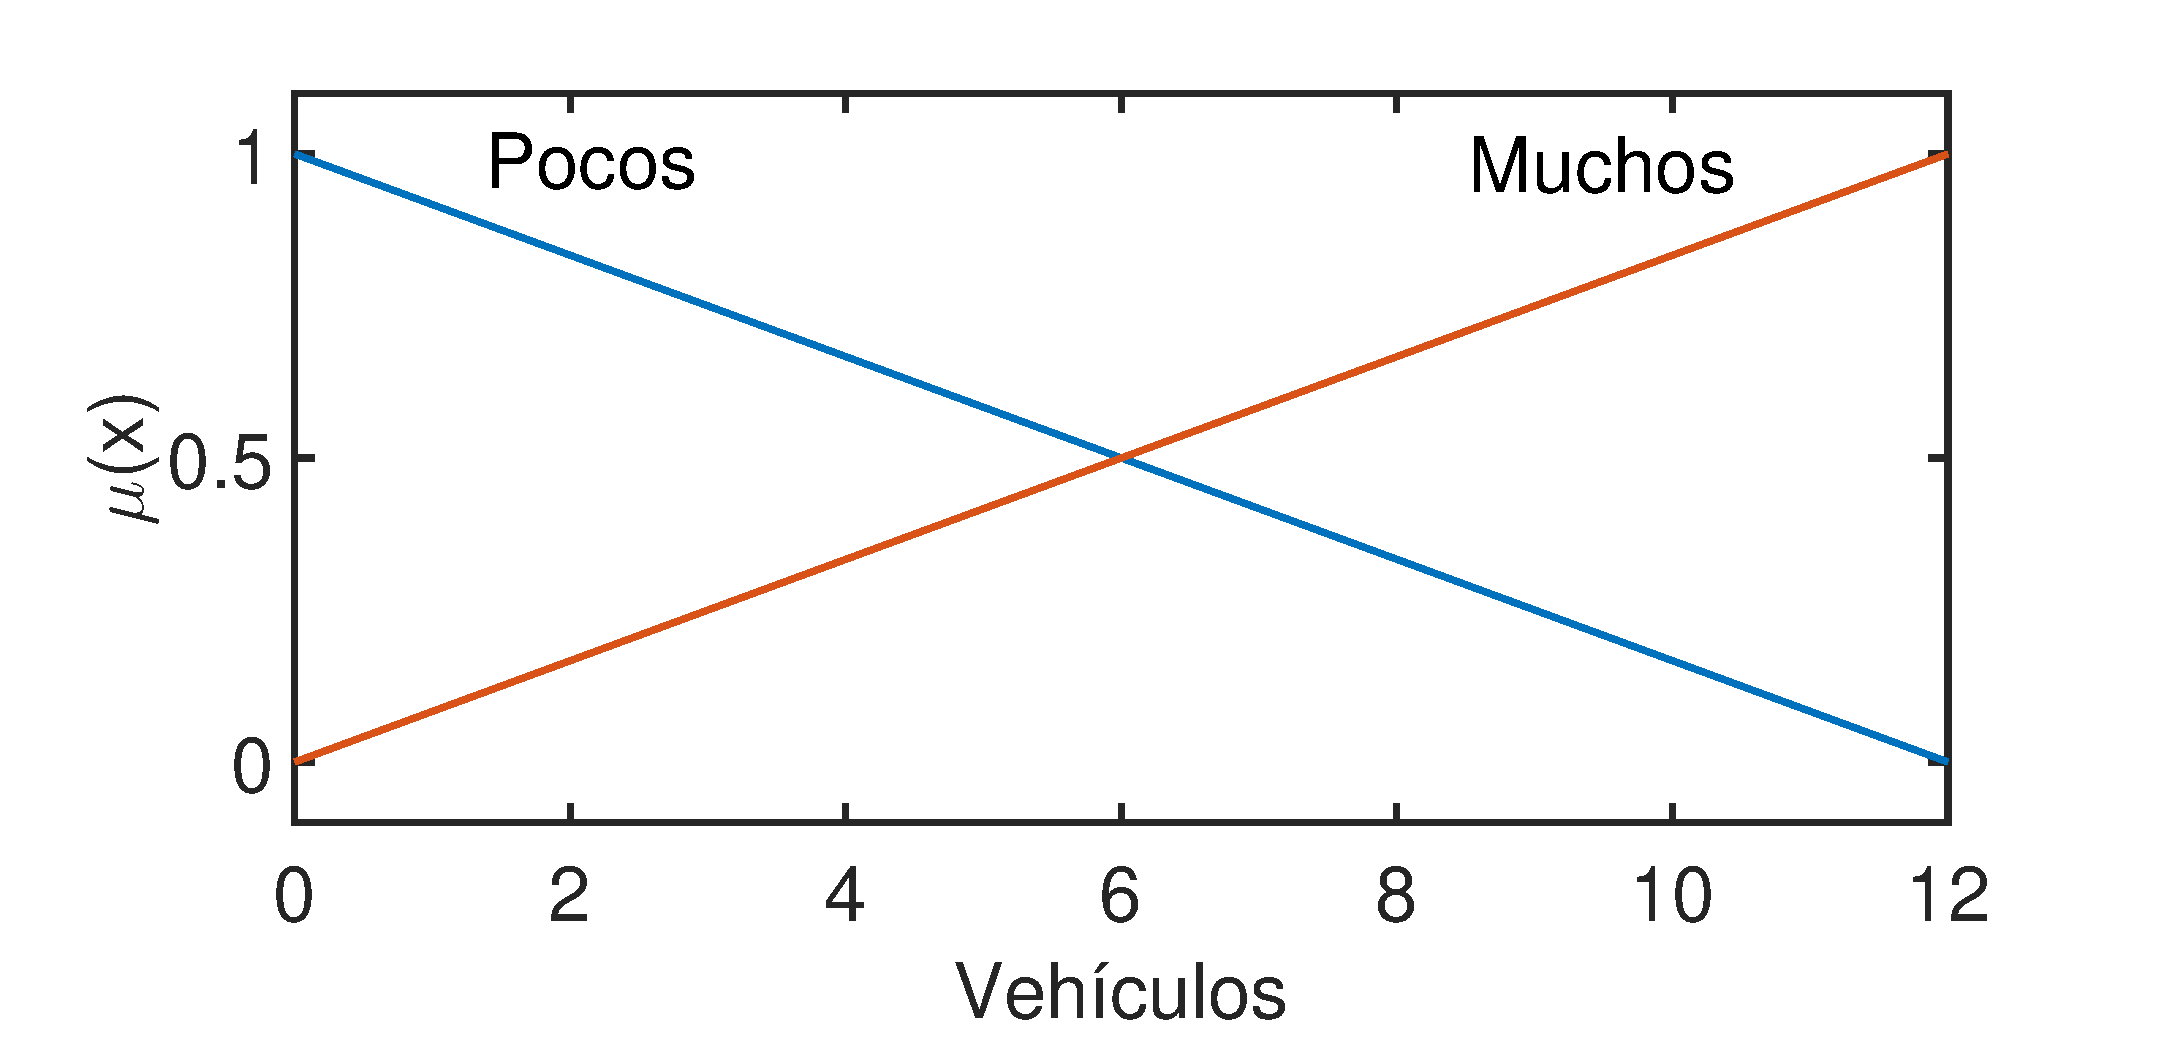
\includegraphics[height=4cm, width=8.1cm]{Variables/ConfigA_input1.eps}}
	\subfigure[Variable lingüística Congestión]{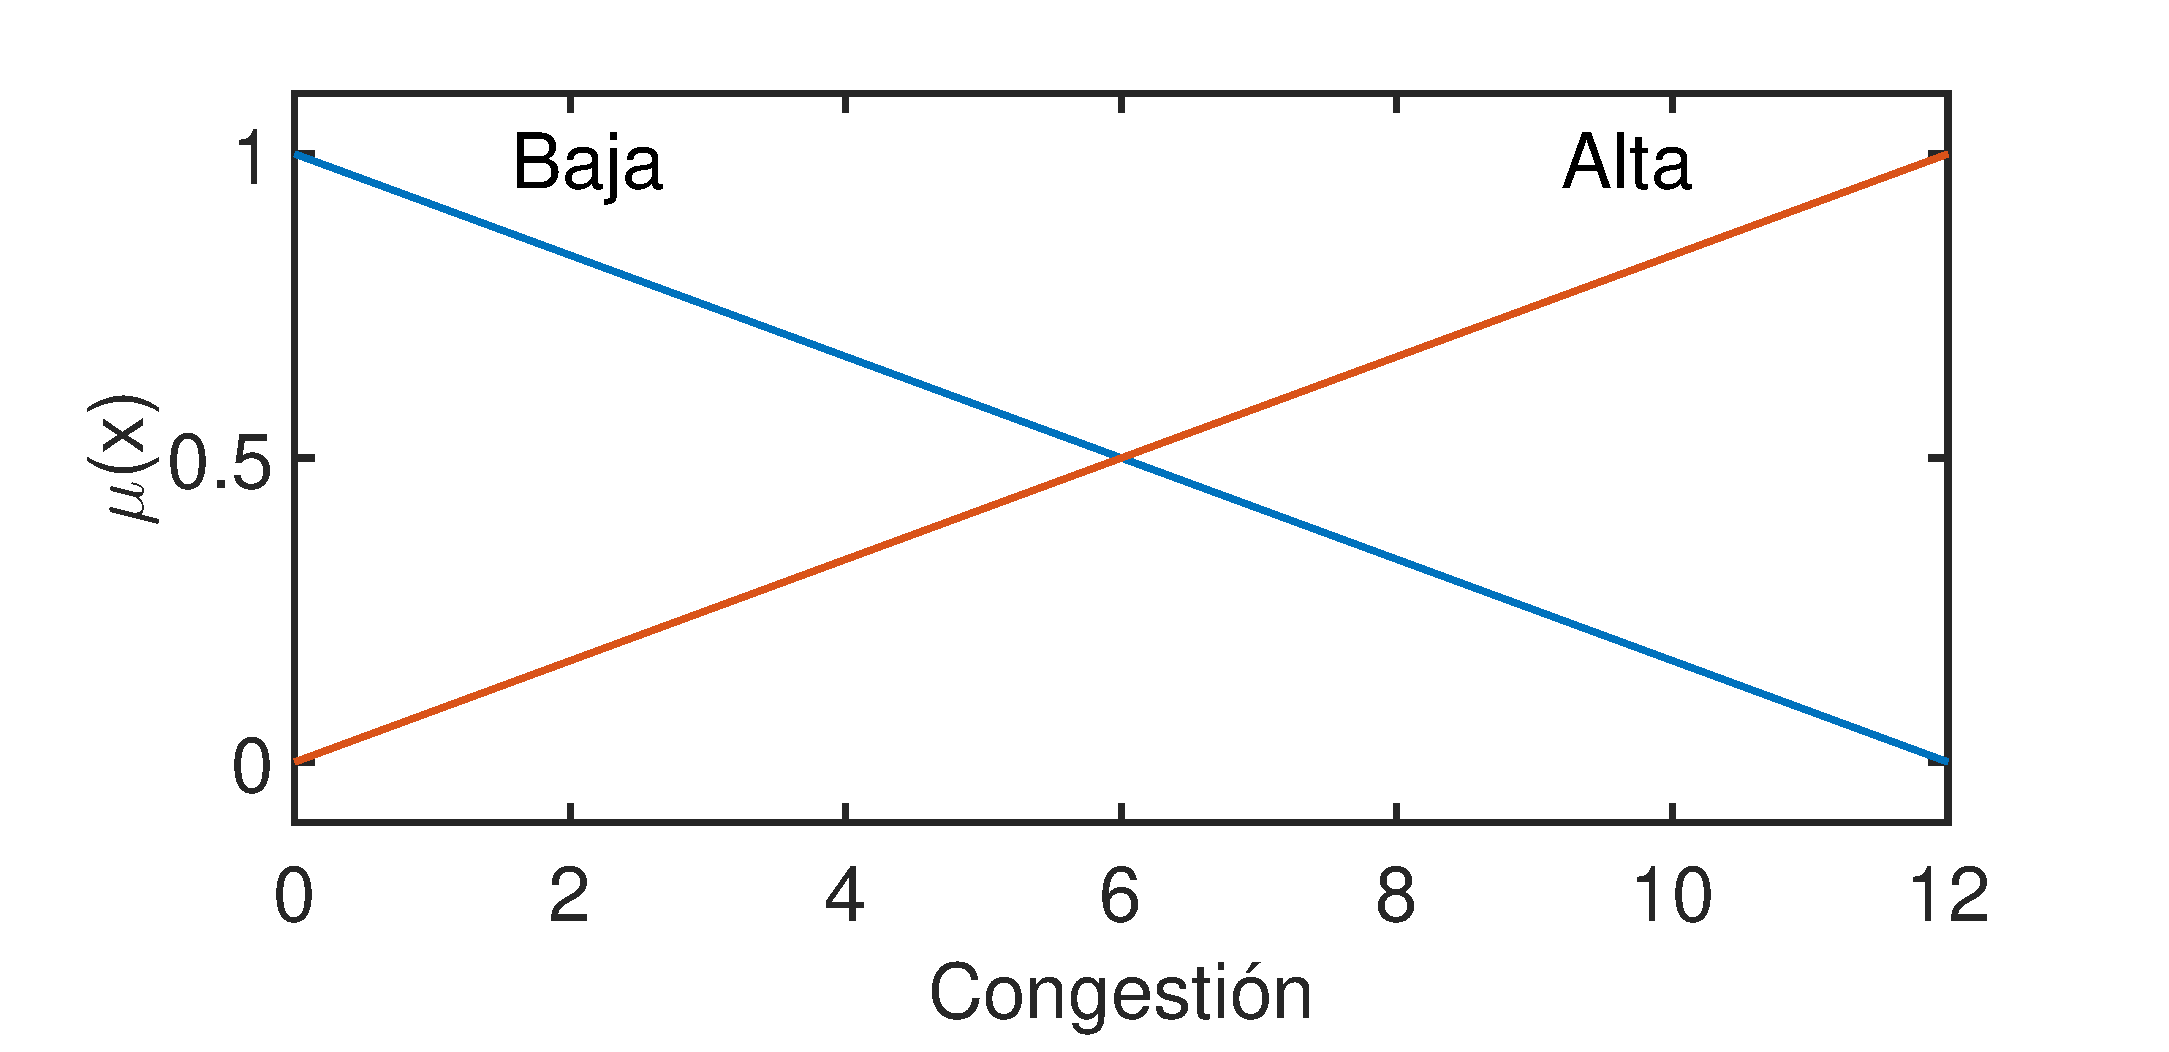
\includegraphics[height=4cm, width=8.1cm]{Variables/ConfigA_input2.eps}}
	\caption[Gráficas de las variables lingüísticas vehículos y congestión]{Representación gráfica de las variables lingüísticas Vehículos y Congestión }
\end{figure}

\pagebreak
\paragraph{Variable de salida Tiempo}
En esta ocasión los parámetros de las funciones de membresía fueron ajustados para generar tiempos más acertados. La nueva configuración de esta variable se muestra a continuación:


\begin{table}[!h]
	\centering
	\begin{tabular}{llr} \toprule
		Termino lingüístico & Función de membresía & Parámetros \\ \midrule
		Bajo & Triangular & [0, 0, 20 ] \\
		Medio & Triangular & [0, 20, 45] \\
		Moderado & Triangular & [20, 45, 70] \\
		Alto & Triangular & [45, 70, 70] \\ \bottomrule
	\end{tabular}
	\caption{Variable lingüística \textit{Tiempo}}
\end{table}

\begin{figure}[H]
	\centering
	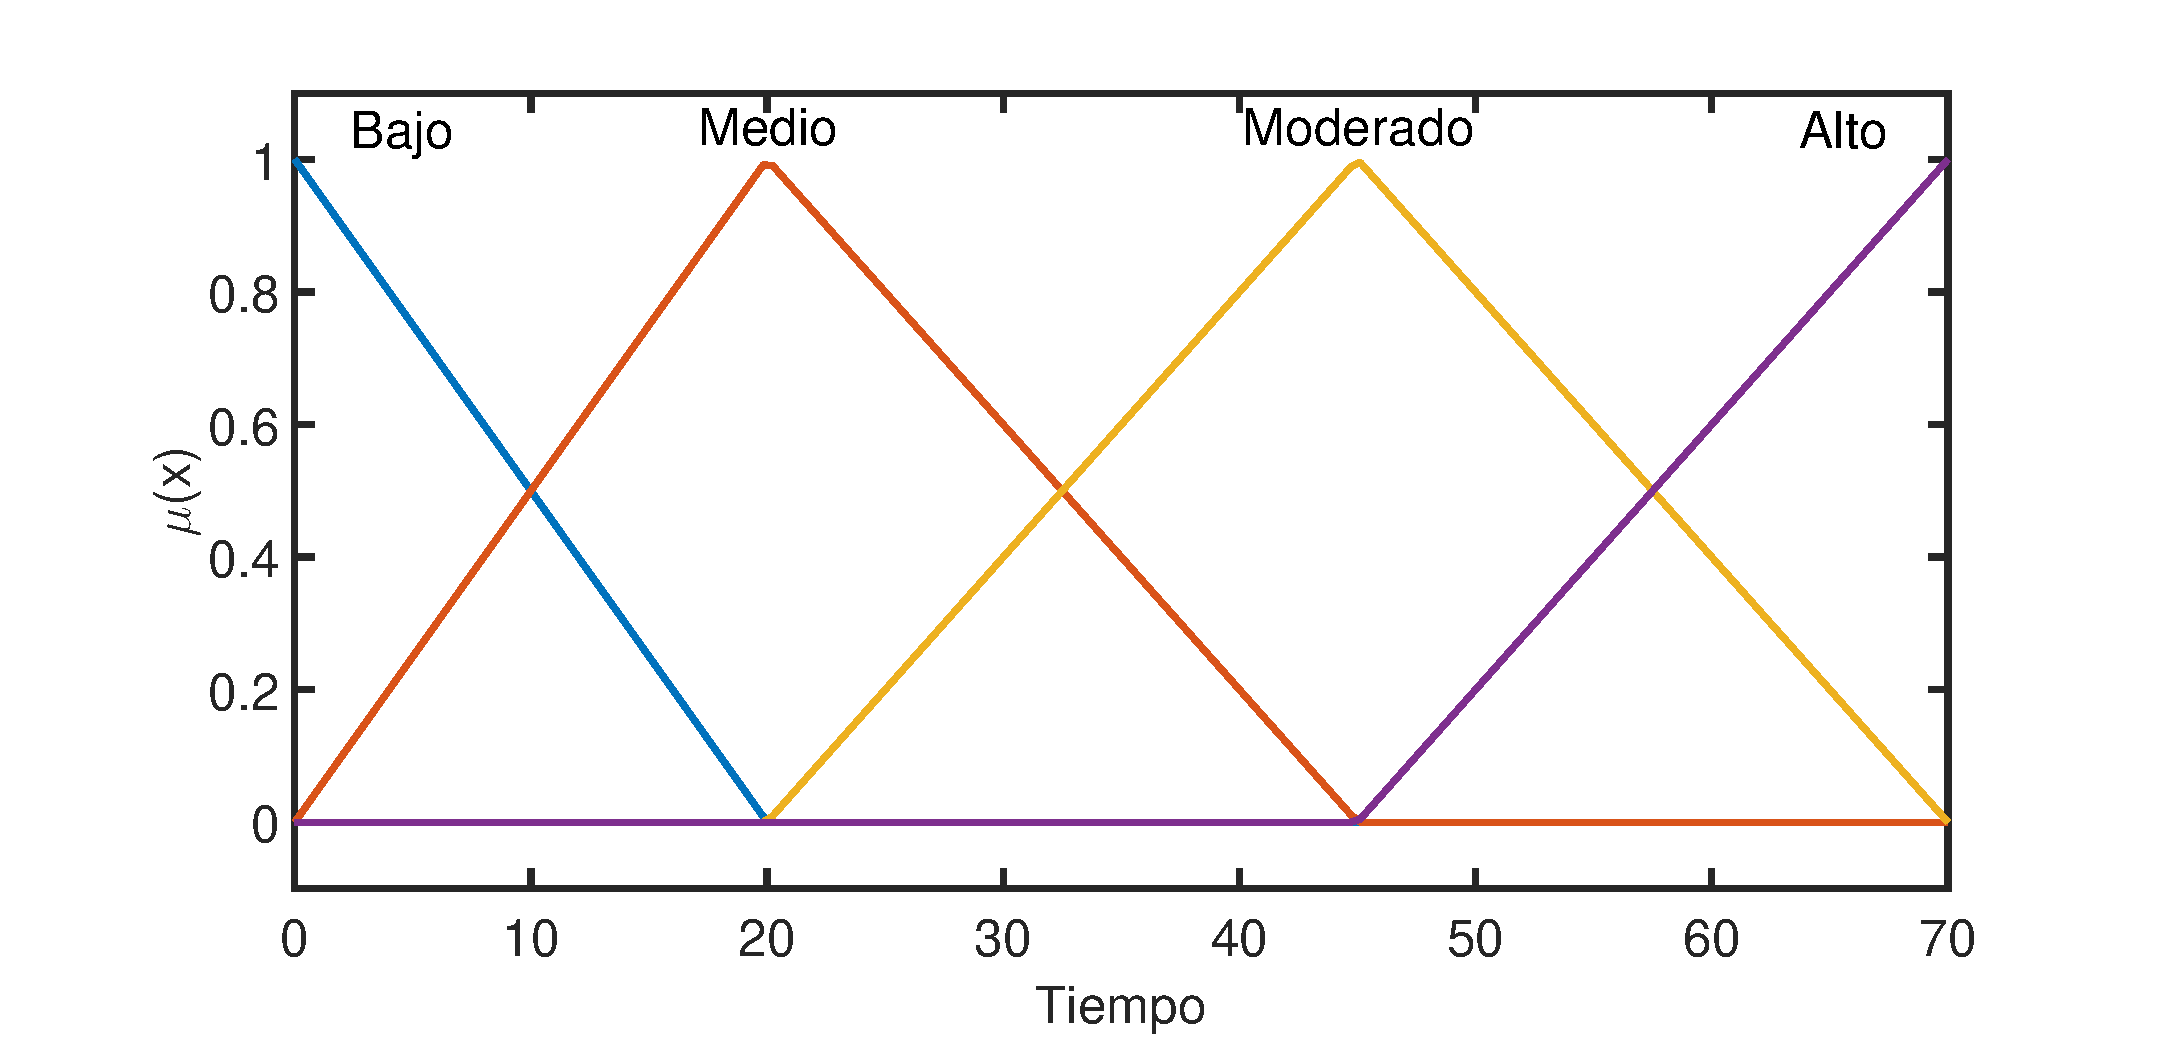
\includegraphics[height=5cm, width=12cm]{Variables/ConfigB_output1.eps}
	\caption[Gráfica variable lingüística tiempo - B]{Representación gráfica de la variable lingüística Tiempo}
\end{figure}

\subsubsection{Base de conocimientos}
La siguiente tabla muestra las reglas difusas empleadas en esta configuración que se mantiene sin cambios.
\begin{longtable}[c]{lclcl} \toprule
	\multicolumn{3}{c}{Antecedente} & & Consecuente \\ \midrule
	Vehículos Pocos & Y & Congestión Baja& $\rightarrow$ & Verde Medio \\
	Vehículos Pocos & Y & Congestión Alta& $\rightarrow$ & Verde Bajo \\
	Vehículos Muchos &Y& Congestión Baja& $\rightarrow$ & Verde Alto \\
	Vehículos Muchos &Y& Congestión Alta& $\rightarrow$ & Verde Moderado \\ \hline
	\caption{Reglas difusas para la configuración \textit{B}}
\end{longtable}

\pagebreak
\subsubsection{Resultados}
Una vez reajustados los parámetros del sistema de inferencia, se le suministraron lo mismos valores de prueba para evaluar su desempeño respecto a la configuración anterior. Los resultados de dicha evaluación se reflejan en la tabla siguiente:

\begin{longtable}[c]{cccccc} \toprule
	$V \backslash C$ &  0 & 3 & 6 & 9 & 12 \\ \midrule
	0 & 21.67 & 21.09 & 19.37 & 15.68 & 06.44 \\
	3 & 29.56 & 29.69 & 29.16 & 28.26 & 27.11 \\
	6 & 35.87 & 35.51 & 35.00 & 34.49 & 34.13 \\
	9 & 43.75 & 42.58 & 40.44 & 39.14 & 39.18 \\
	12& 61.90 & 52.60 & 48.15 & 45.83 & 45.00 \\
	\caption{Resultados de la evaluación para la configuración \textit{B}}
\end{longtable}

Donde: la columna V son los valores de prueba de la variable Vehículos, la fila C son los valores de  prueba de la variable Congestión y las celdas son los tiempos (en segundos) obtenidos por la configuración actual.

\subsubsection{Observaciones}
\begin{multicols}{2}
Después de evaluar el desempeño de la segunda configuración se observa como efectivamente el tiempo asignado es más acorde a la cantidad de vehículos; sin embargo, el tiempo asignado para las entradas Vehículos = 0 y Congestión = 0, resulta generoso puesto que la cantidad de vehículos a los que se les cederá el paso es mínimo (0) mientras al igual que el índice de vehículos (6); Sería mejor que en estos casos el tiempo fuera más corto para acelerar el ciclo del semáforo y reducir la espera de las otras avenidas. En otro casos como V = 12 y C = 12, el tiempo podría resultar insuficiente para desahogar el tráfico, por lo que se ajustará en la siguiente configuración.

\begin{figure}[H]
	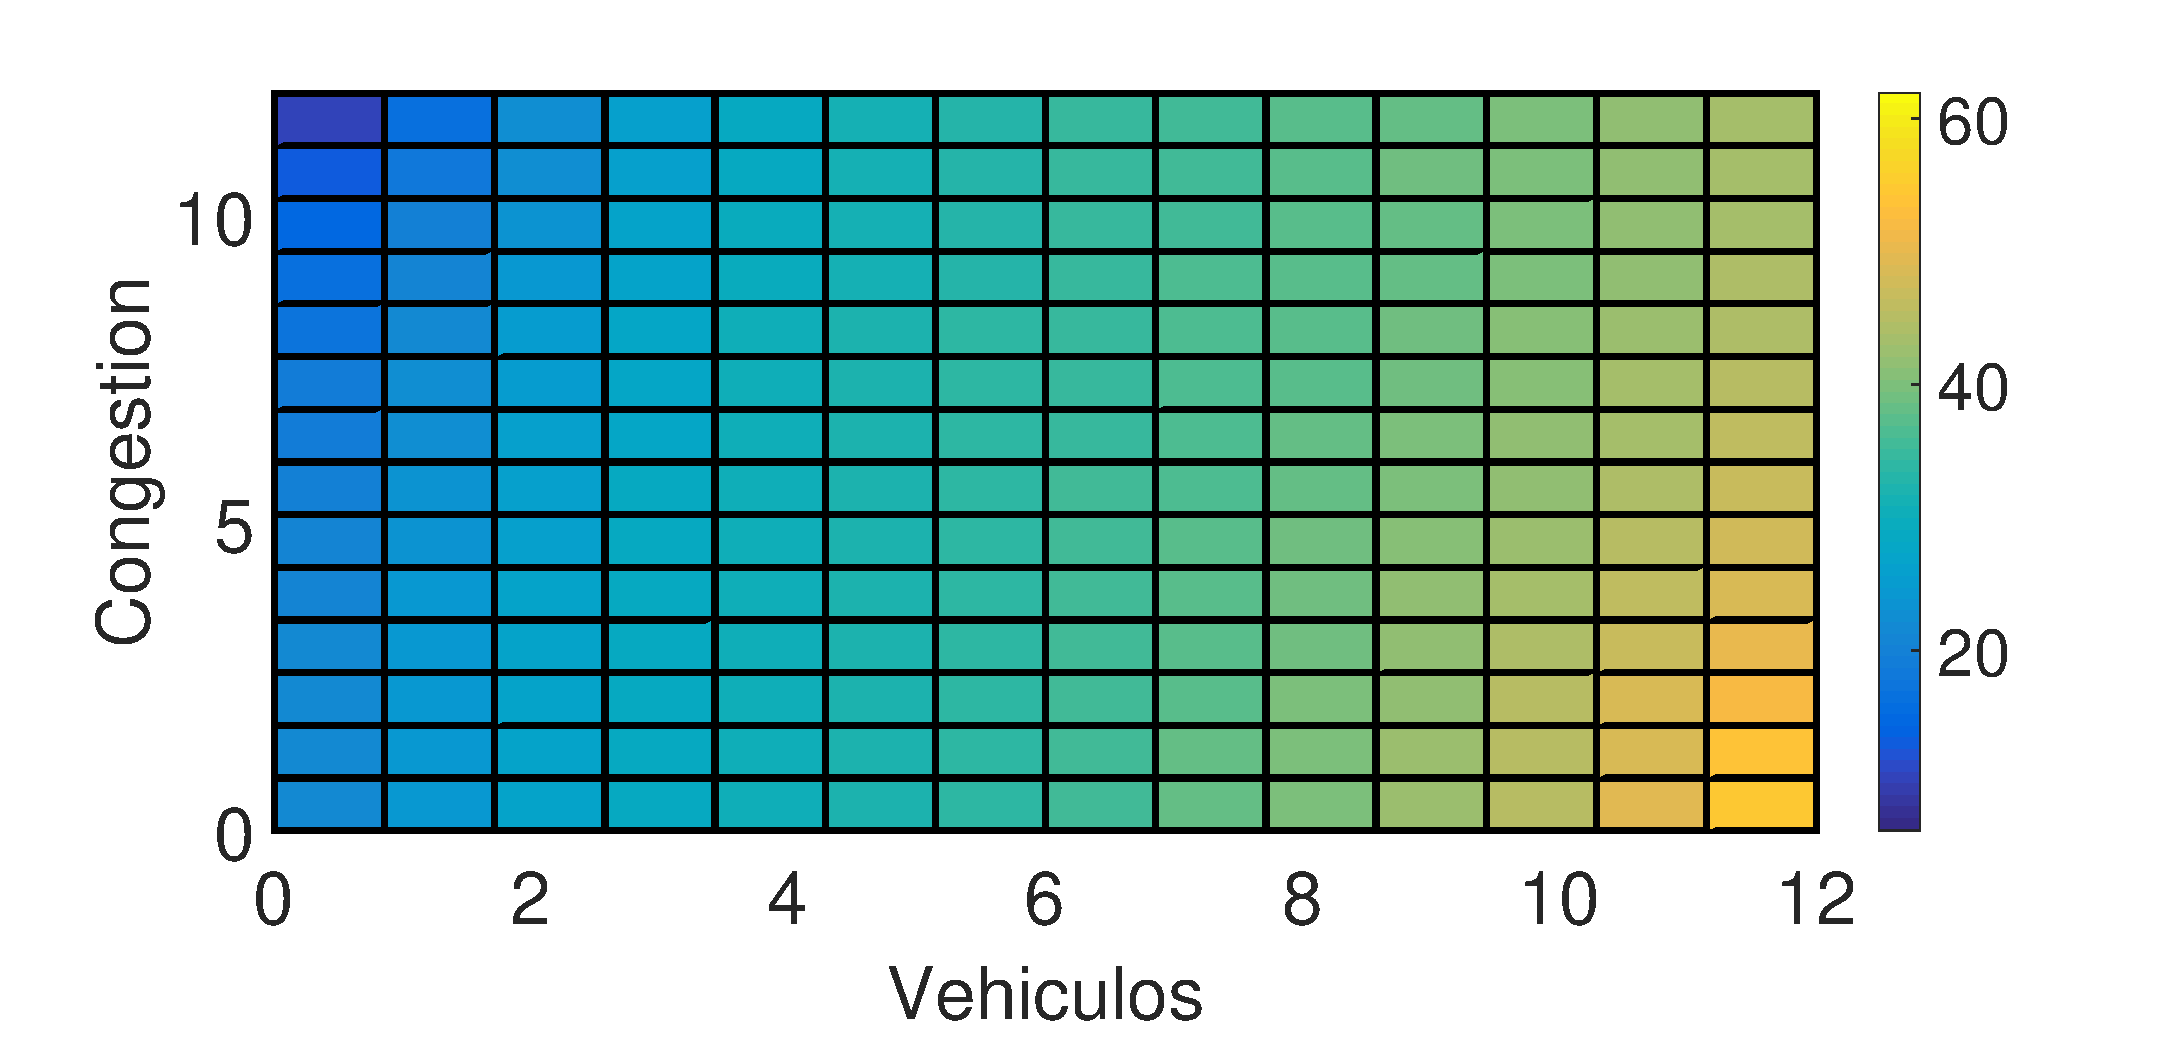
\includegraphics[width=0.5\textwidth]{Surfaces/Surface2D_B.eps}
	\caption{Superficie de control}
\end{figure}

\end{multicols}


\pagebreak
\subsection{Configuración C}
En está ocasión los reajustes serán mayores a los de la configuración anterior. Puesto que se agregaran un nuevo termino lingüístico a las variables Vehículos y Tiempo.

\paragraph{Variable de entrada Vehículos} Se agrega un nuevo término lingüístico para aumentar la flexibilidad del sistema.

\begin{table}[!h]
	\centering
	\begin{tabular}{llr} \toprule
		Termino lingüístico & Función de membresía & Parámetros \\ \midrule
		Pocos & Triangular & [0, 0, 6 ] \\
		Moderados & Triangular & [0, 6, 12 ] \\
		Muchos & Triangular & [6, 12, 12] \\ \bottomrule
	\end{tabular}
	\caption{Variable lingüística \textit{Vehículos}}
\end{table}


\paragraph{Variable de entrada Congestión} se mantiene sin cambios desde la configuración anterior.


\begin{table}[!h]
	\centering
	\begin{tabular}{llr} \toprule
		Termino lingüístico & Función de membresía & Parámetros \\ \midrule
		Baja & Triangular & [0, 0, 12 ] \\
		Alta & Triangular & [0, 12, 12] \\ \bottomrule
	\end{tabular}
	\caption{Variable lingüística \textit{Congestión}}
\end{table}

\begin{figure}[H]
	\centering
	\subfigure[Variable lingüística Vehículos]{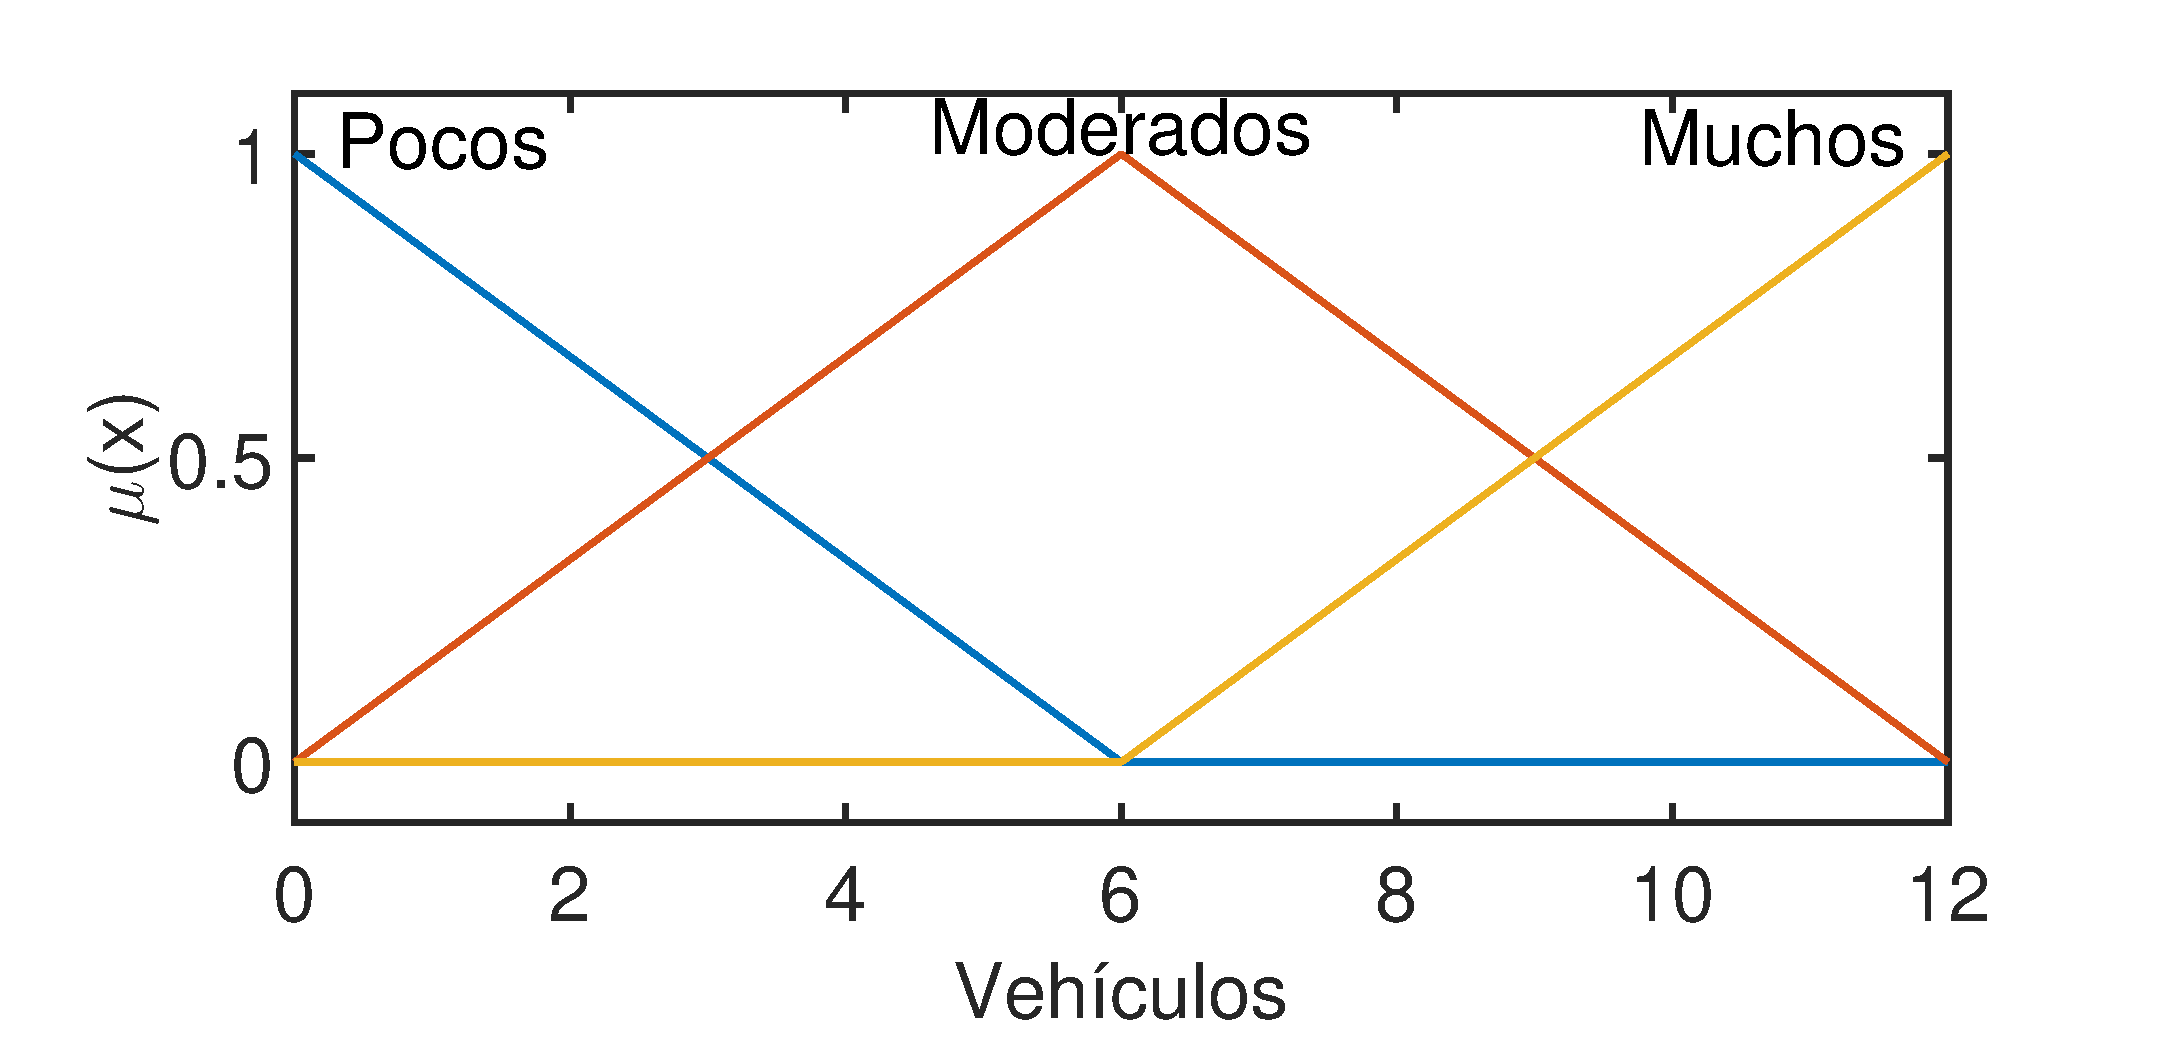
\includegraphics[height=4cm, width=8.1cm]{Variables/ConfigC_input1.eps}}
	\subfigure[Variable lingüística Congestión]{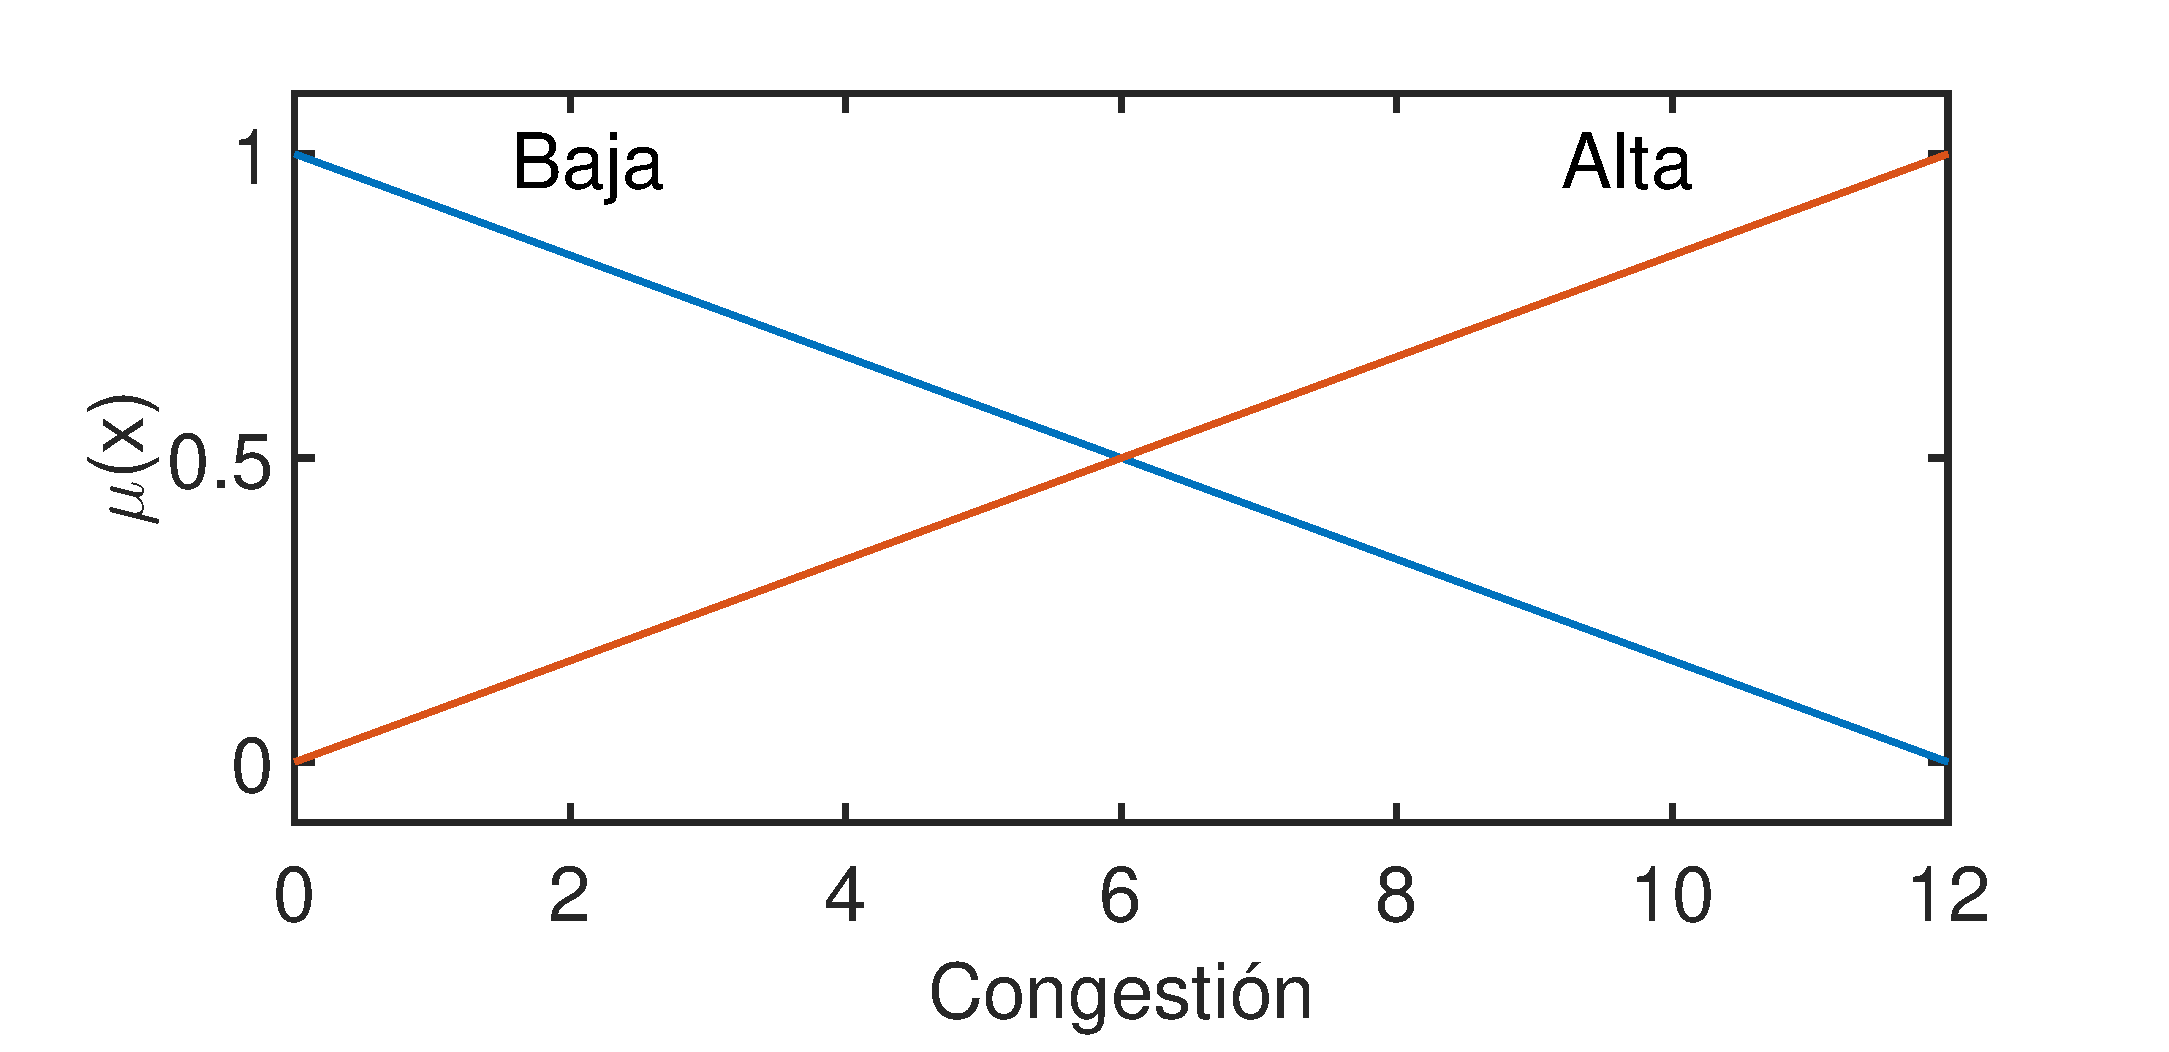
\includegraphics[height=4cm, width=8.1cm]{Variables/ConfigA_input2.eps}}
	\caption[Gráficas de las variables lingüísticas vehículos y congestión]{Representación gráfica de las variables lingüísticas Vehículos y Congestión }
\end{figure}

\pagebreak
\paragraph{Variable de salida Tiempo} al igual que la variable vehículos, se ha agregado un nuevo término lingüístico para aumentar la flexibilidad. Además los parámetros de las funciones fueron reajustados ligeramente al igual que sus etiquetas.

\begin{table}[!h]
	\centering
	\begin{tabular}{llr} \toprule
		Termino lingüístico & Función de membresía & Parámetros \\ \midrule
		Mínimo & Triangular & [0, 10, 20 ] \\
		Bajo & Triangular & [0, 20, 40 ] \\
		Medio & Triangular & [20, 40, 60] \\
		Alto & Triangular & [40, 60, 80] \\
		Extra & Triangular & [60, 80, 80] \\ \bottomrule
	\end{tabular}
	\caption{Variable lingüística \textit{Tiempo}}
\end{table}

\begin{figure}[H]
	\centering
	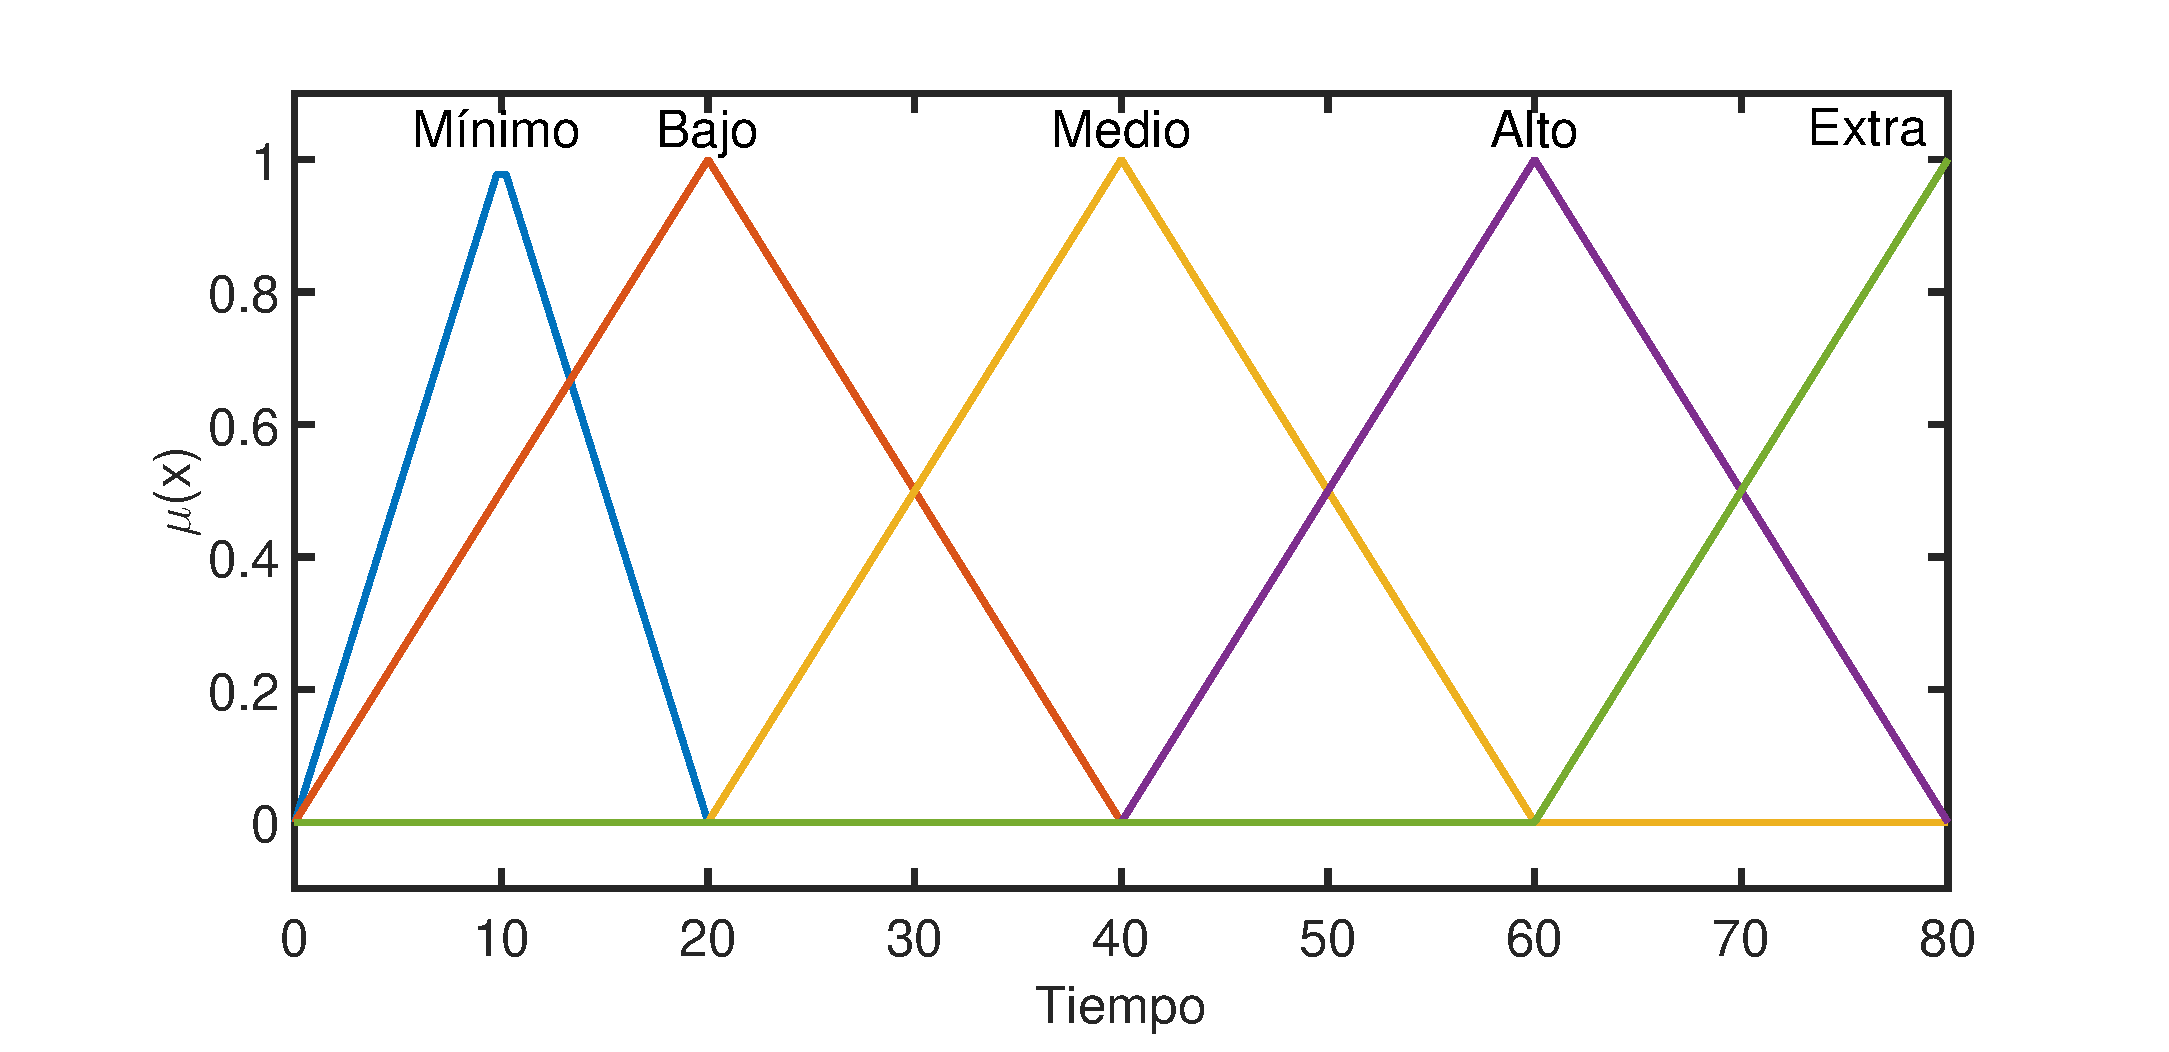
\includegraphics[height=5cm, width=12cm]{Variables/ConfigC_output1.eps}
	\caption[Gráfica variable lingüística tiempo - C]{Representación gráfica de la variable lingüística Tiempo}
\end{figure}

\subsubsection{Base de conocimientos}
La siguiente tabla muestra las reglas difusas empleadas en esta configuración que se mantiene sin cambios.
\begin{longtable}[c]{lclcl} \toprule
	\multicolumn{3}{c}{Antecedente} & & Consecuente \\ \midrule
	\multicolumn{3}{c}{Vehículos Pocos} & $\rightarrow$ & Verde Mínimo \\
	Vehículos Moderados & Y & Congestión Baja& $\rightarrow$ & Verde Medio \\
	Vehículos Moderados & Y & Congestión Alta& $\rightarrow$ & Verde Bajo \\
	Vehículos Muchos &Y& Congestión Baja& $\rightarrow$ & Verde Extra \\
	Vehículos Muchos &Y& Congestión Alta& $\rightarrow$ & Verde Alto \\ \hline
	\caption{Reglas difusas para la configuración \textit{C}}
\end{longtable}

\pagebreak
\subsubsection{Resultados}
Una vez reajustados los parámetros del sistema de inferencia, se le suministraron lo mismos valores de prueba para evaluar su desempeño respecto a la configuración anterior. Los resultados de dicha evaluación se reflejan en la tabla siguiente:

\begin{longtable}[c]{cccccc} \toprule
	$V \backslash C$ &  0 & 3 & 6 & 9 & 12 \\ \midrule
	0 & 10.00 & 10.00 & 10.00 & 10.00 & 10.00 \\
	3 & 30.00 & 29.63 & 28.81 & 25.59 & 18.85 \\
	6 & 40.00 & 34.21 & 30.00 & 25.79 & 20.00 \\
	9 & 59.74 & 44.49 & 42.44 & 40.75 & 40.00 \\
	12& 73.33 & 65.87 & 62.38 & 60.59 & 60.00 \\
	\caption{Resultados de la evaluación para la configuración \textit{C}}
\end{longtable}

Donde: la columna V son los valores de prueba de la variable Vehículos, la fila C son los valores de  prueba de la variable Congestión y las celdas son los tiempos (en segundos) obtenidos por la configuración actual.

\subsubsection{Observaciones}
\begin{multicols}{2}

	En esta tercera configuración se aprecia que hubo mejoras considerables en los tiempos inferidos por el sistema. Si se observa la salida para V = 12 y C = 12, cuya salida es 60, se nota que es un tiempo bastante acertado que ayudaría a desahogar la congestión. Por otro lado cuando V = 12 y C = 0, el sistema otorga 13 segundos extra. En el caso contrario, cuando V = 0 y C = 12, el sistema asigna el tiempo mínimo de 10 segundos. Hace falta un nuevo ajuste para saber si los tiempos pueden mejorar aún más.
	
	\begin{figure}[H]
		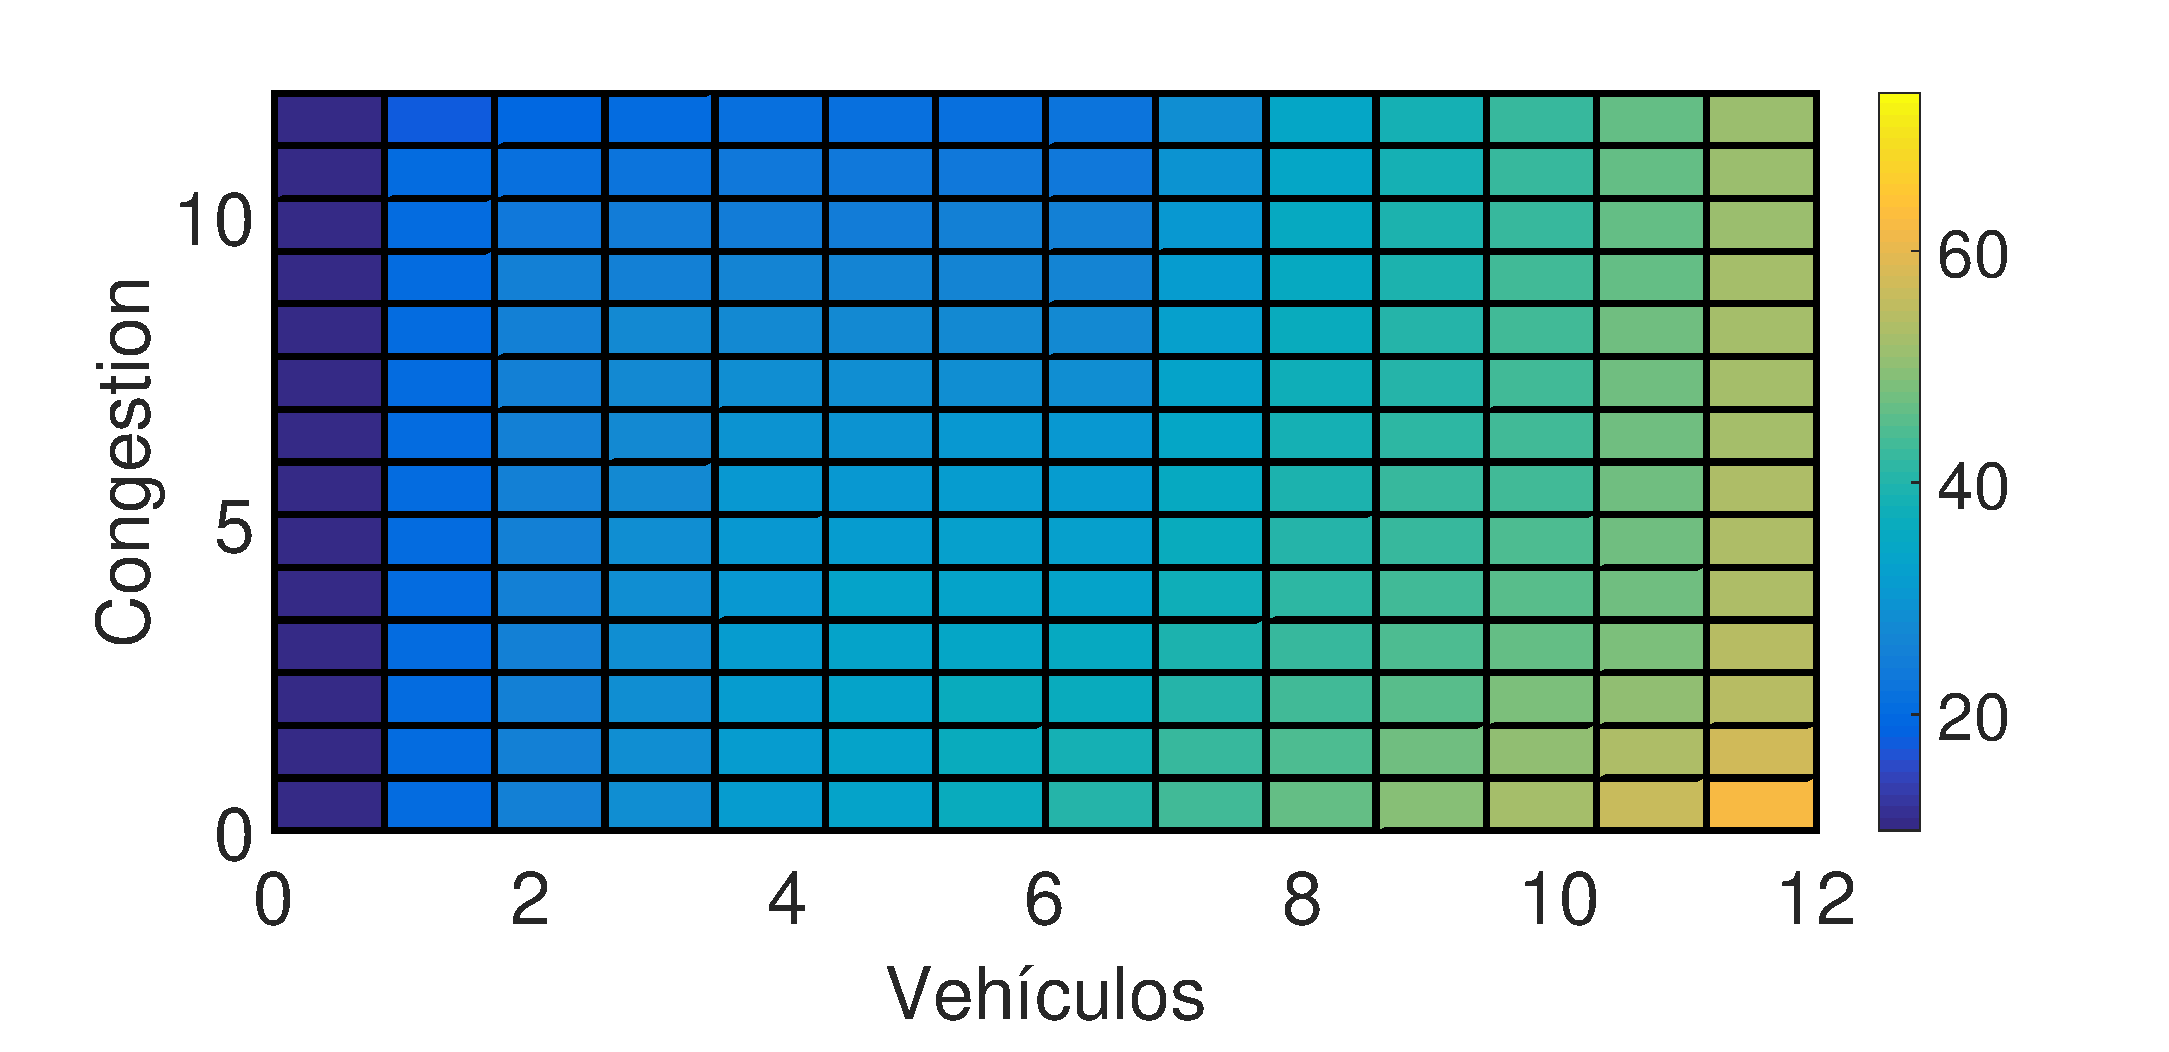
\includegraphics[width=0.5\textwidth]{Surfaces/Surface2D_C.eps}
		\caption{Superficie de control}
	\end{figure}
\end{multicols}
\pagebreak





\subsection{Configuración D}\label{section:configd}
Existen funciones de membresía que modelan mejor el modo de clasificación que realiza la mente humana, estas funciones son las curvas tales como: \textit{Sigmoidales, Gaussianas y Campanas Generalizadas}; en esta configuración se explota el potencial de las primeras dos.

\paragraph{Variable de entrada Vehículos} las funciones de membresía \textit{triangulares} se remplazan por funciones \textit{Sigmoidales y Gaussianas}, estás modelan de manera más eficiente la manera en que el ser humano suele clasificar los fenómenos.
\begin{center}
	\begin{tabular}{llr} \toprule
		Termino lingüístico & Función de membresía & Parámetros \\ \midrule
		Pocos & Sigmoidal & [ -0.8, 4 ] \\
		Moderados & Gaussiana & [ 1.6, 7 ] \\
		Muchos & Sigmoidal & [ 0.8, 10] \\ \bottomrule
	\end{tabular}
	\captionof{table}{Variable lingüística \textit{Vehículos}}
\end{center}

\paragraph{Variable de entrada Congestión} también se remplaza las funciones triangulares por \textit{funciones Sigmoidales}.

\begin{table}[!h]
	\centering
	\begin{tabular}{llr} \toprule
		Termino lingüístico & Función de membresía & Parámetros \\ \midrule
		Baja & Sigmoidal & [ -0.8, 5 ] \\
		Alta & Sigmoidal & [ 0.8, 5 ] \\ \bottomrule
	\end{tabular}
	\caption{Variable lingüística \textit{Congestión}}
\end{table}
\begin{figure}[H]
	\centering
	\subfigure[Variable lingüística Vehículos]{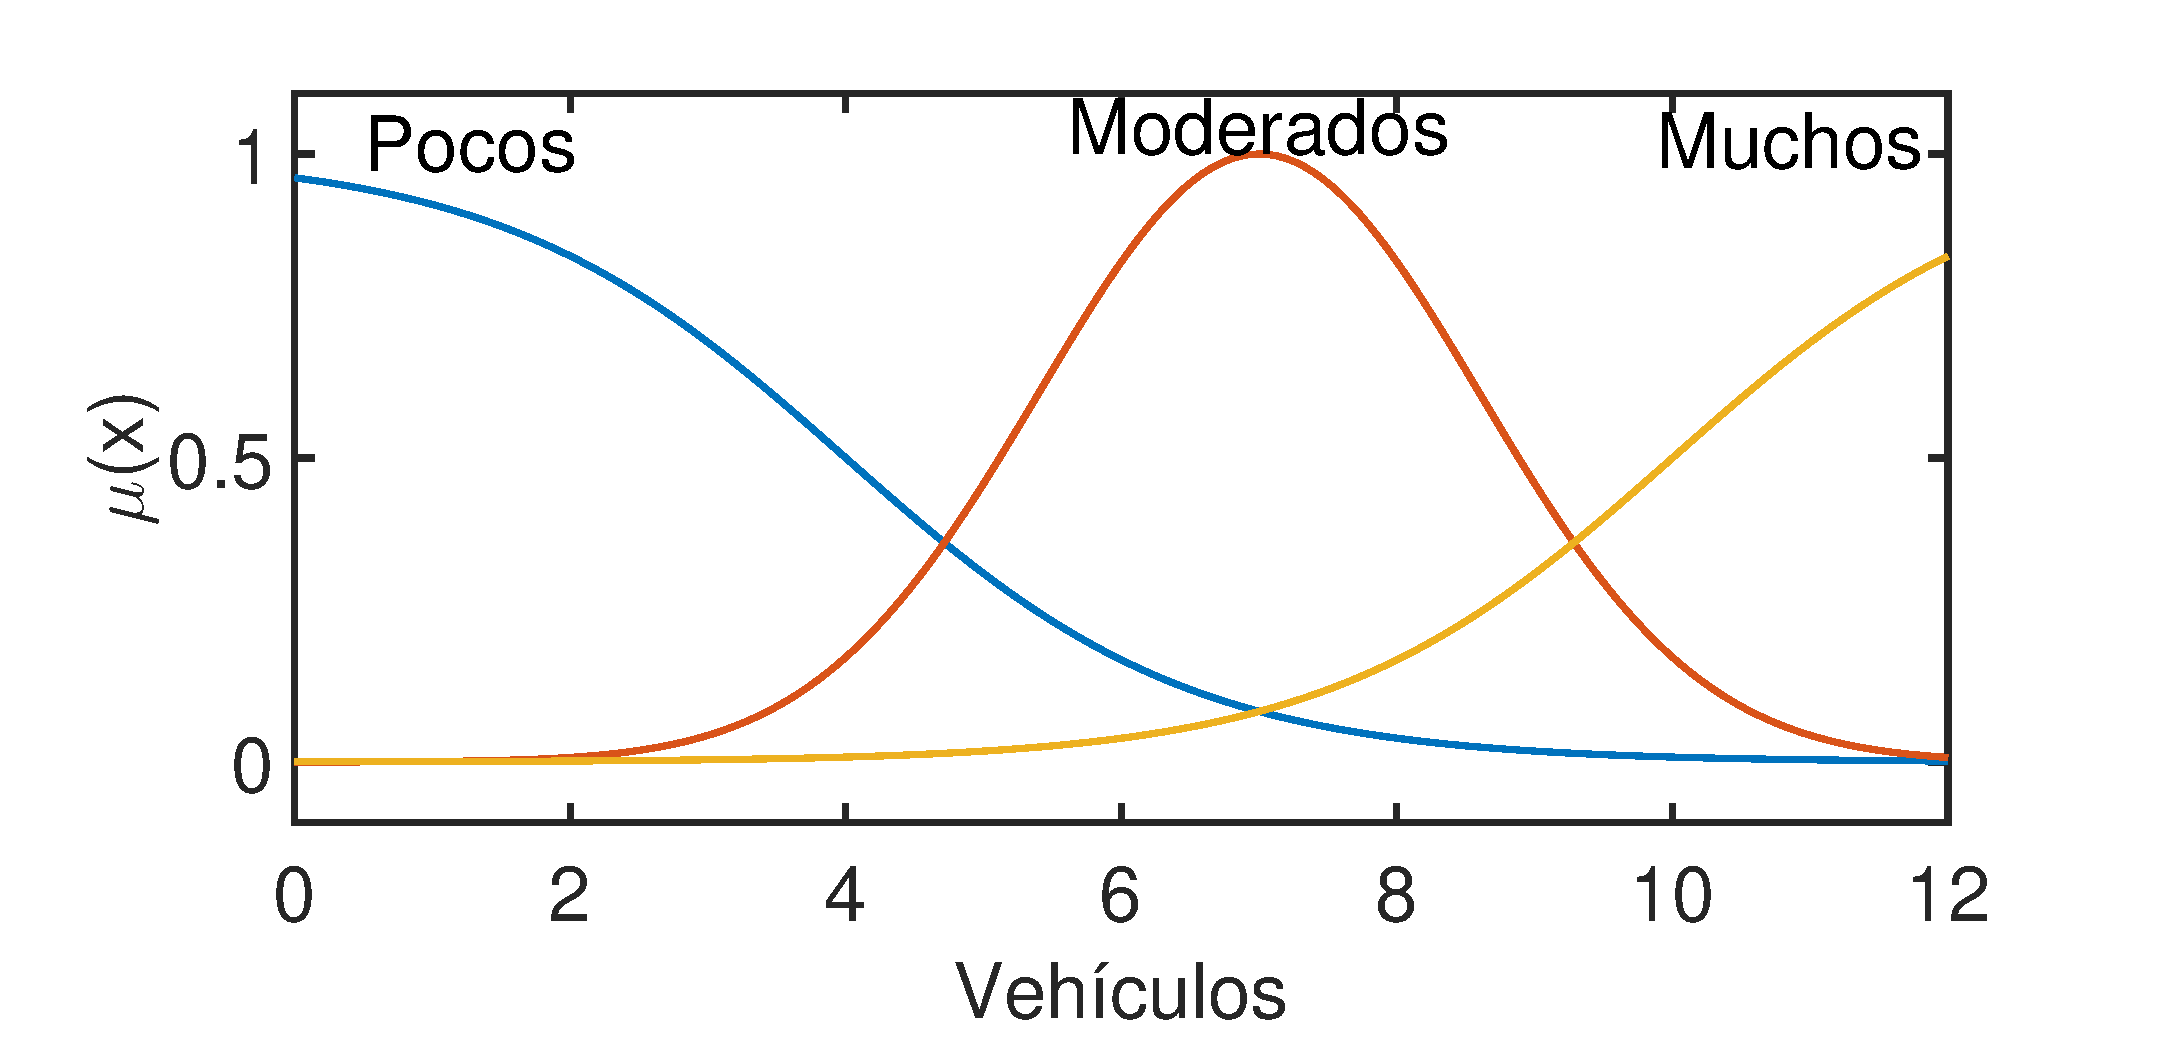
\includegraphics[height=4cm, width=8.1cm]{Variables/ConfigD_input1.eps}}
	\subfigure[Variable lingüística Congestión]{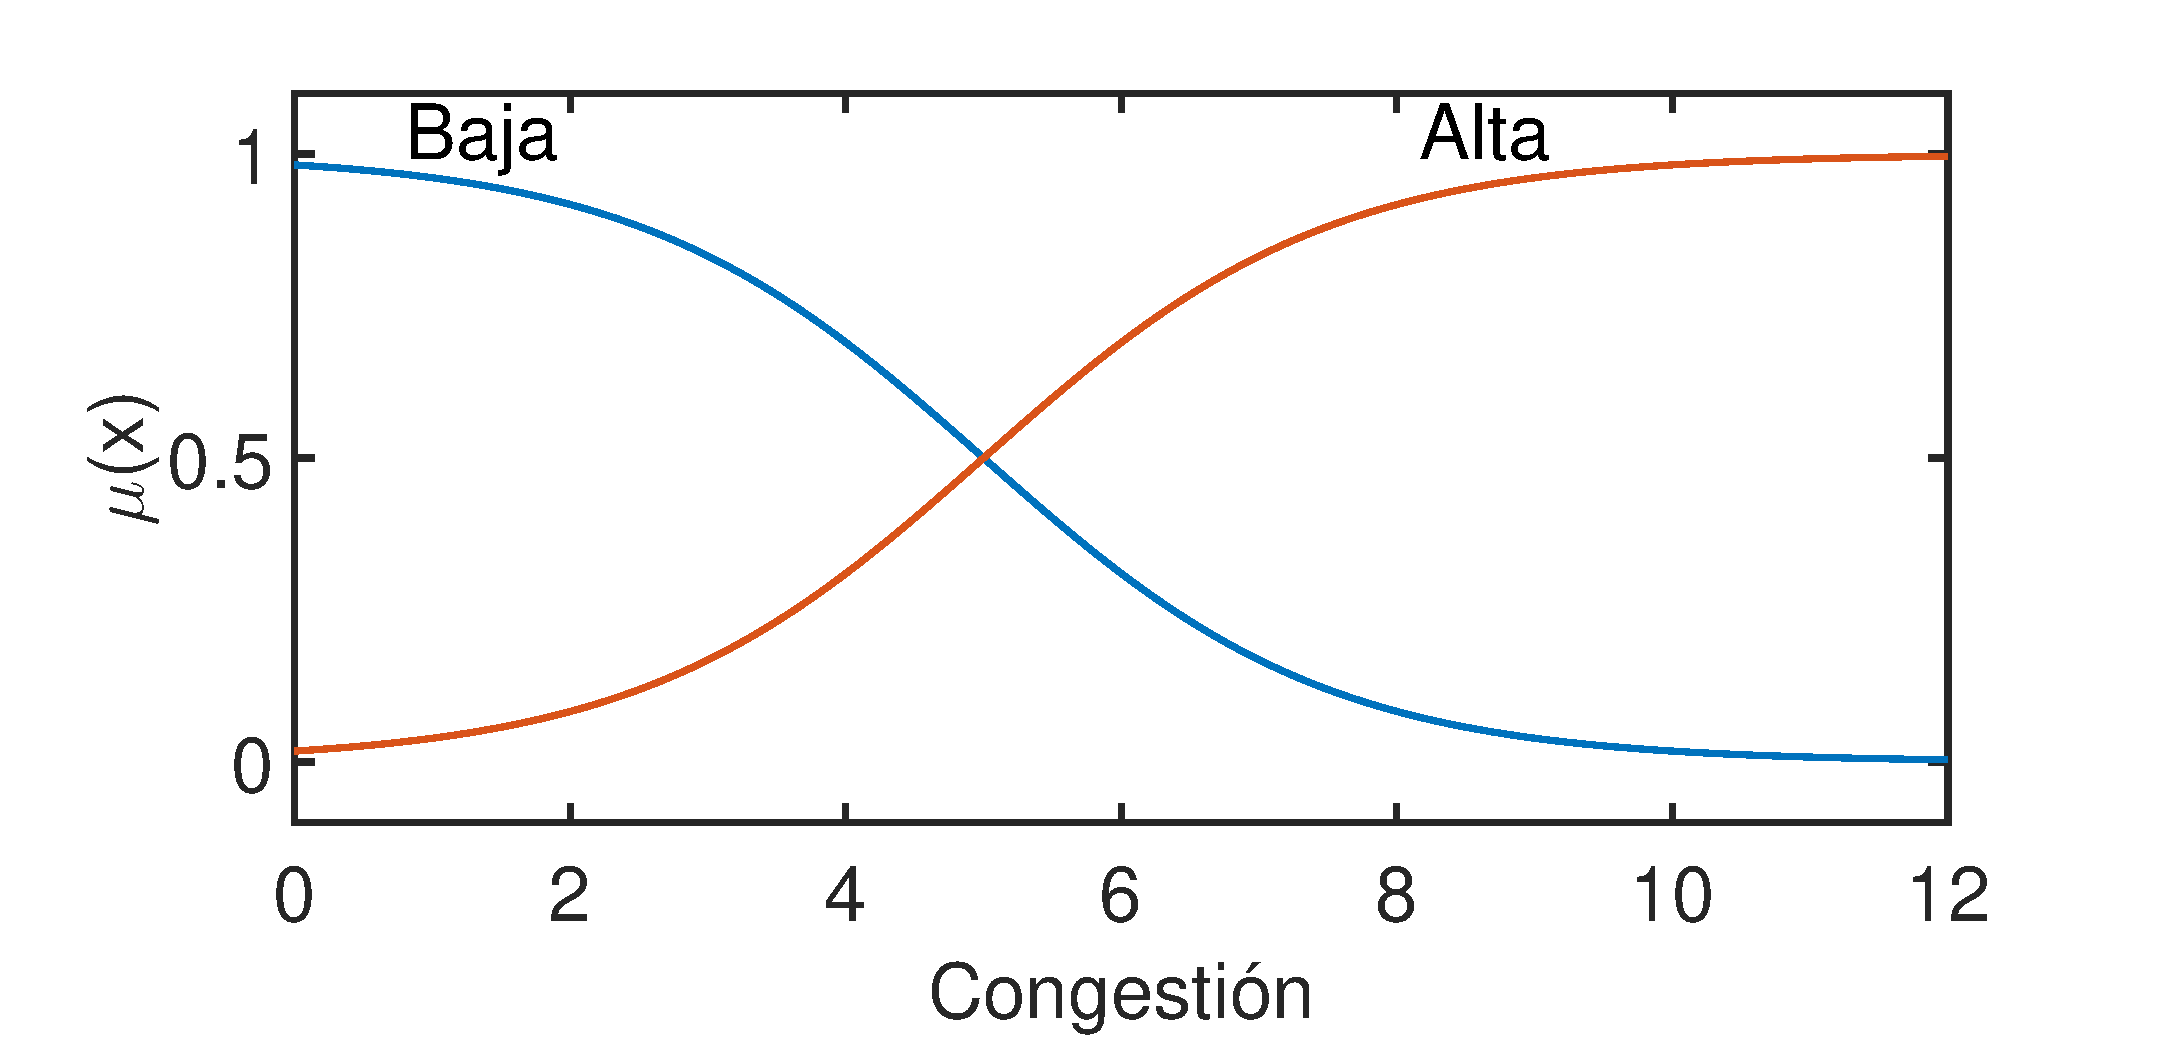
\includegraphics[height=4cm, width=8.1cm]{Variables/ConfigD_input2.eps}}
	\caption[Gráficas de las variables lingüísticas vehículos y congestión]{Representación gráfica de las variables lingüísticas Vehículos y Congestión }
\end{figure}

\paragraph{Variable de salida Tiempo} esta variable únicamente tiene un ajuste menor en el término lingüístico \textit{Mínimo}, el resto de términos permanece intacto.

\begin{table}[!h]
	\centering
	\begin{tabular}{llr} \toprule
		Termino lingüístico & Función de membresía & Parámetros \\ \midrule
		Mínimo & Triangular & [0, 0, 25 ] \\
		Bajo & Triangular & [0, 25, 40 ] \\
		Medio & Triangular & [20, 40, 60] \\
		Alto & Triangular & [40, 60, 80] \\
		Extra & Triangular & [60, 80, 80] \\ \bottomrule
	\end{tabular}
	\caption{Variable lingüística \textit{Tiempo}}
\end{table}

\begin{figure}[H]
	\centering
	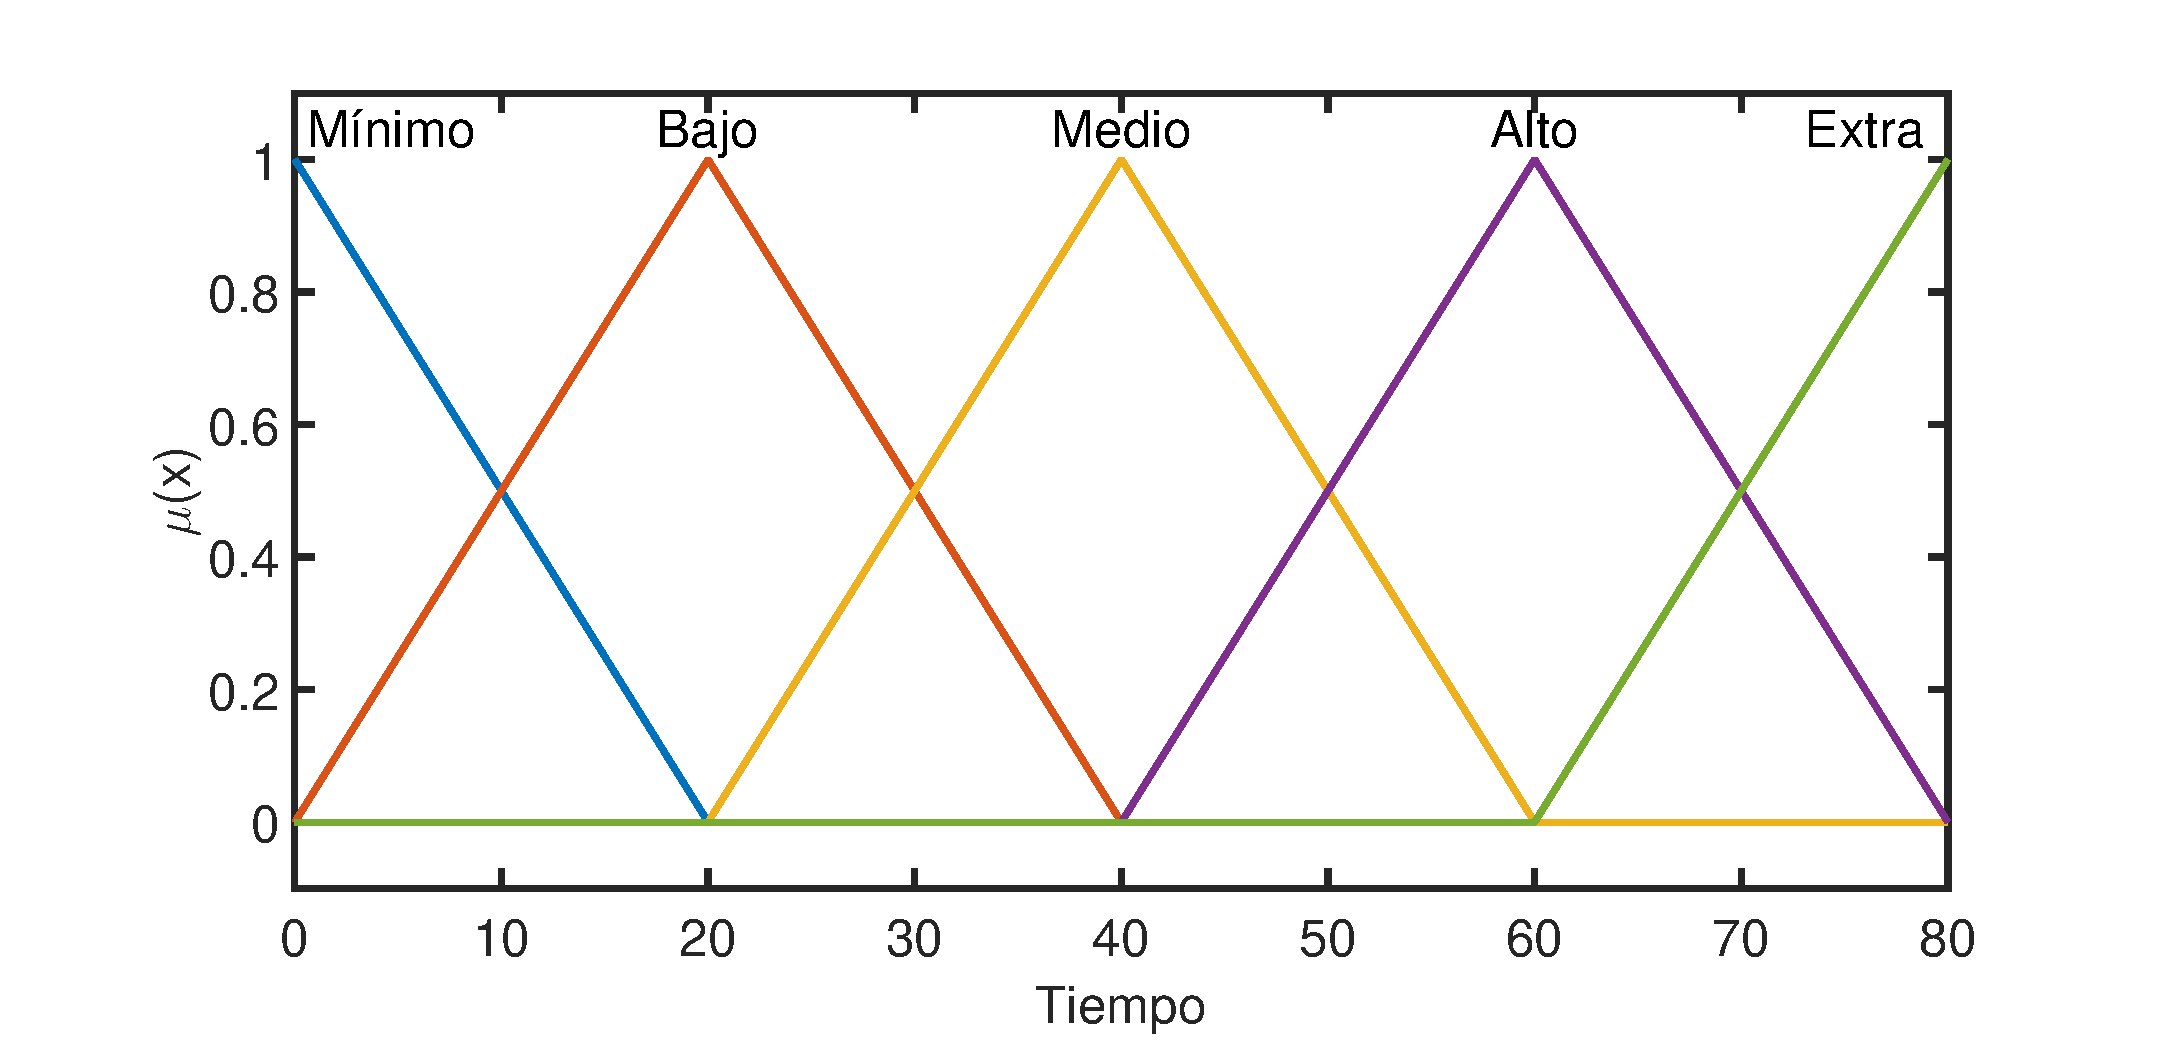
\includegraphics[height=5cm, width=12cm]{Variables/ConfigD_output1.eps}
	\caption[Gráfica variable lingüística tiempo - D]{Representación gráfica de la variable lingüística Tiempo}
\end{figure}

\subsubsection{Base de conocimientos}
La siguiente tabla muestra las reglas difusas empleadas en esta configuración que se mantiene sin cambios.
\begin{longtable}[c]{lclcl} \toprule
	\multicolumn{3}{c}{Antecedente} & & Consecuente \\ \midrule
	\multicolumn{3}{c}{Vehículos Pocos} & $\rightarrow$ & Verde Mínimo \\
	Vehículos Moderados & Y & Congestión Baja& $\rightarrow$ & Verde Medio \\
	Vehículos Moderados & Y & Congestión Alta& $\rightarrow$ & Verde Bajo \\
	Vehículos Muchos &Y& Congestión Baja& $\rightarrow$ & Verde Extra \\
	Vehículos Muchos &Y& Congestión Alta& $\rightarrow$ & Verde Alto \\ \hline
	\caption{Reglas difusas para la configuración \textit{D}}
\end{longtable}

\pagebreak
\subsubsection{Resultados}
Después de remplazar algunas de las funciones de membresía y realizar los ajustes necesarios, se le suministró los mismos valores de prueba para evaluar su desempeño respecto a la configuración anterior. Los resultados de dicha evaluación se reflejan en la tabla siguiente:

\begin{longtable}[c]{cccccc} \toprule
	$V \backslash C$ &  0 & 3 & 6 & 9 & 12 \\ \midrule
	0 & 08.41 & 08.41 & 08.41 & 08.41 & 08.41 \\
	3 & 13.25 & 13.25 & 13.25 & 12.98 & 10.85 \\
	6 & 36.56 & 36.54 & 28.81 & 24.08 & 24.02 \\
	9 & 47.81 & 43.60 & 39.23 & 37.65 & 37.62 \\
	12& 70.83 & 66.58 & 60.27 & 59.40 & 59.39 \\
	\caption{Resultados de la evaluación para la configuración \textit{D}}
\end{longtable}

Donde: la columna V son los valores de prueba de la variable Vehículos, la fila C son los valores de  prueba de la variable Congestión y las celdas son los tiempos (en segundos) obtenidos por la configuración actual.

\subsubsection{Observaciones}

\begin{multicols}{2}
	Definitivamente, los resultados obtenidos tras remplazar las funciones triangulares por funciones sigmoidales y gaussianas, son mucho más acertadas. Al principio, los tiempos asignados incrementan más rápido conforme más se eleva el número de autos, después, el ritmo de crecimiento de los tiempos de asignación desacelera al acercarse al valor máximo para las variables de entrada. Se concluye que la configuración actual será la usada en la implementación.
	\begin{figure}[H]
	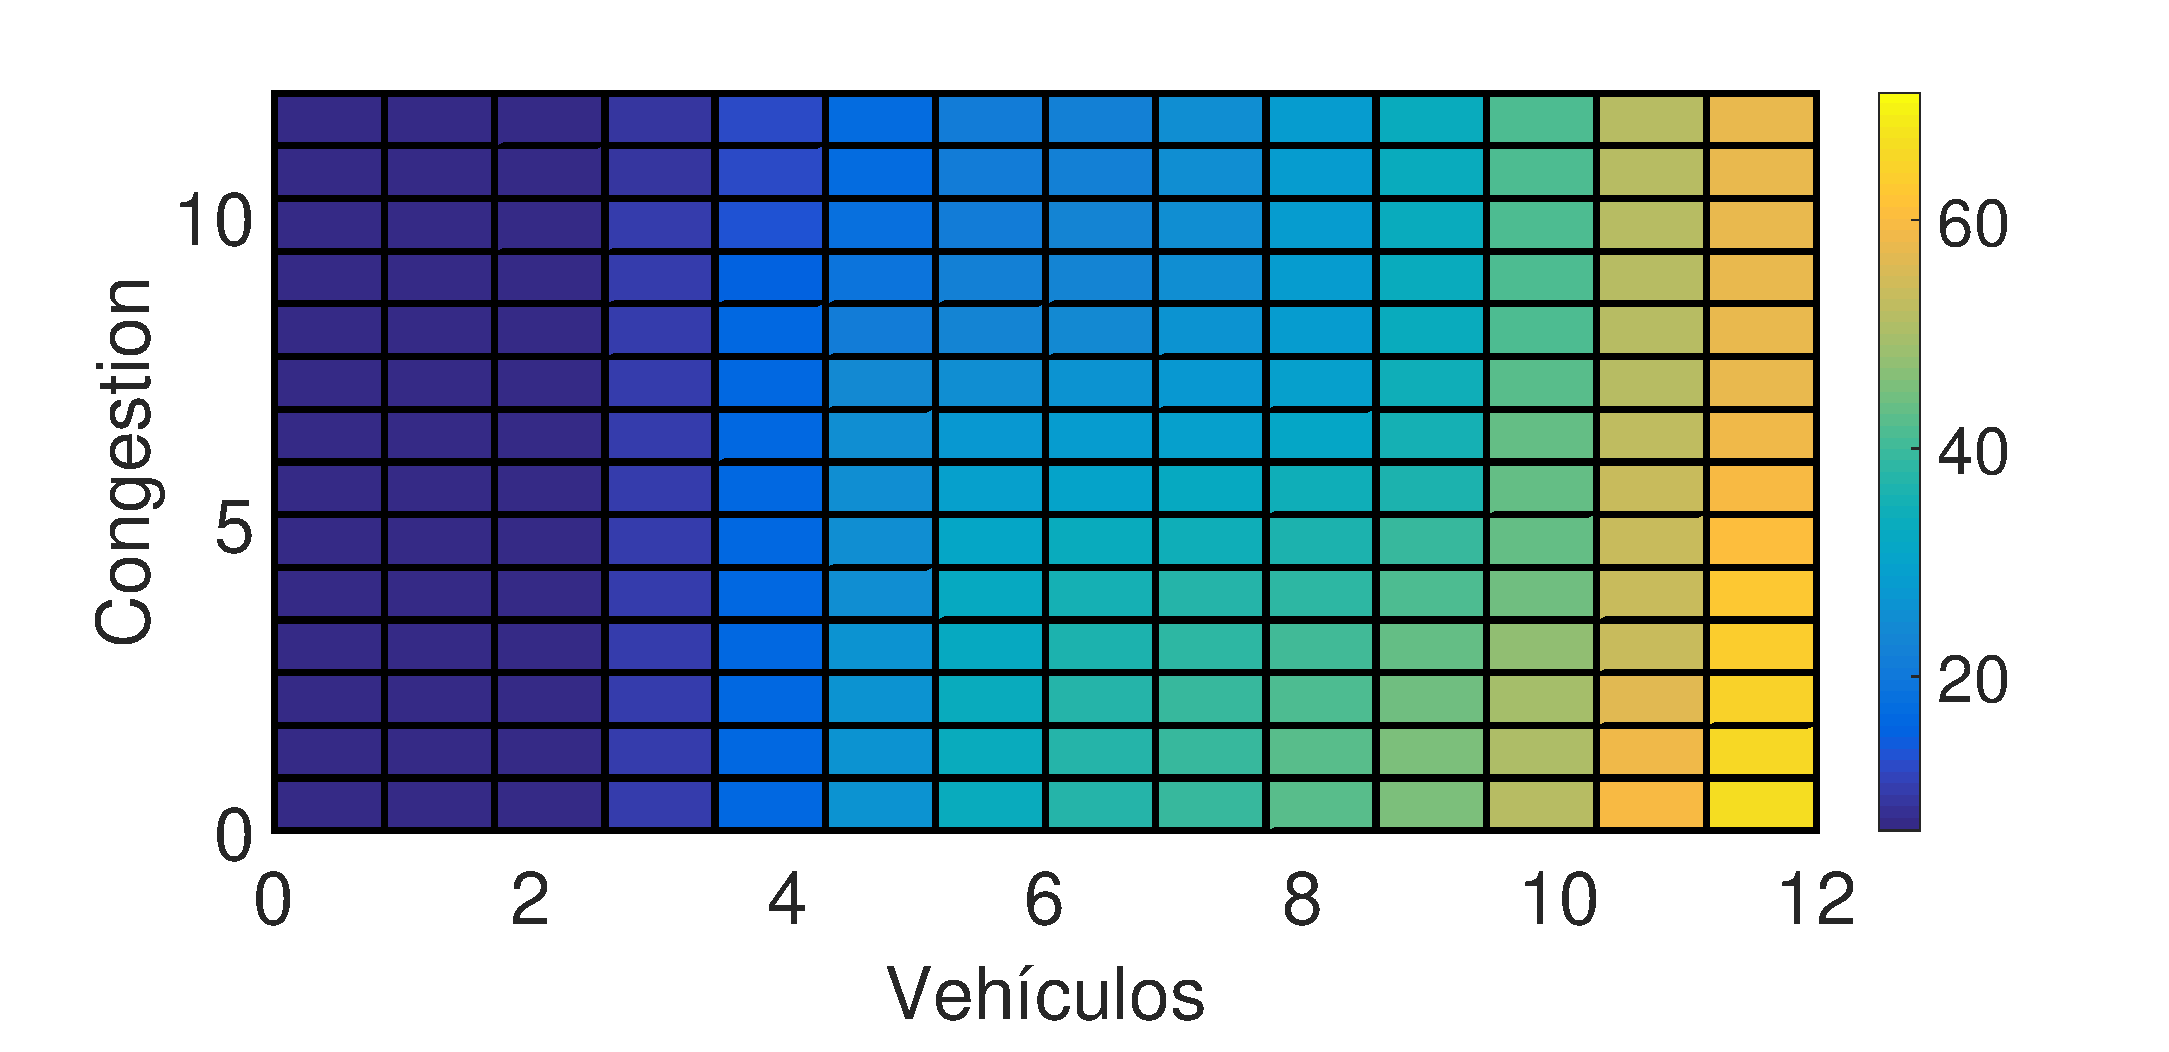
\includegraphics[width=0.5\textwidth]{Surfaces/Surface2D_D.eps}
	\caption{Superficie de control}
\end{figure}
\end{multicols}
\pagebreak

\section{Desarrollo del algoritmo}\label{section:desarrolloAlgoritmo}
Después de haber culminado el desarrollo del sistema de inferencia, el cual representa el componente principal del proyecto, ahora el desarrollo continúa con el algoritmo de sincronización de semáforos.

El modelo propuesto, es a su vez un marco de trabajo para la implementación última, por parte del usuario final.

A lo largo de las siguientes páginas se modela el desarrollo del algoritmo mediante diagramas UML, empleando solo aquellos diagramas que ayuden a tener una perspectiva general del proyecto.
\begin{itemize}
	\item Diagrama de Actividades del flujo general del sistema
	\item Diagrama de Clases de todo el sistema
	\item Diagrama de Secuencia del bucle principal
\end{itemize}

\begin{figure}[H]
	\centering
	\begin{tikzpicture}
	[node distance=10mm and 15mm,
	 legend/.style={pos=0.4, font=\scriptsize, fill=white},
	 block/.style={rectangle,draw=black,fill=yellow!20,thin,minimum height=10mm, minimum width=43mm, font=\footnotesize},
	 rline/.style={->, shorten >= 1pt, >= stealth', semithick,draw=black},]
	 	\node[block] (cam) {Sensor Vehiculos {\scriptsize (e.g. Cámara)} };
		\node[block] (in) [below=of cam] {Entradas {\scriptsize (e.g. Congestión)}};
		\node[block] (fis) [below=of in] {Sistema Difuso};
		\node[block] (out) [below=of fis] {Salidas {\scriptsize (e.g. Tiempo)}};
		\node[block] (sem) [below=of out] {Semáforo ``Inteligente''};

		\node[block] (rules) [left=of fis] {Reglas Difusas};
		\node[block] (vars) [right=of fis] {Variables Lingüísticas};

		\draw [rline] (cam) -- node[legend] {Pre-Procesamiento} (in);
		\draw [rline] (in) -- node[legend] {Fuzzificación} (fis);
		\draw [rline] (fis) -- node[legend] {Defuzzificación} (out);
		\draw [rline] (out) -- node[legend] {Post-Procesamiento} (sem);
		
		\draw [rline] (rules) -- (fis);
		\draw [rline] (vars) -- (fis);
	\end{tikzpicture}
	\caption{Diagrama general del sistema}
\end{figure}

\newpage
\subsection{Diagrama de actividades}
El siguiente diagrama muestra a grandes rasgos, el flujo de ejecución general del algoritmo. En él se puede observar el proceso de inicialización y configuración del semáforo y del sensor; además se muestra el bucle principal ``\emph{repetir siempre}'' que se encarga de obtener los datos del sensor, procesarlos y establecer el cambio de fase.

\begin{figure}[H]
	\centering
	\begin{tikzpicture}
		[auto,
		decision/.style	={diamond, draw=blue, thin, fill=yellow!20, text width=5cm, align=flush center, inner sep=1pt},
		bucle/.style	={chamfered rectangle, draw=black, thin, fill=yellow!20, text width=5.5cm, align=flush center, minimum height=2em},
		block/.style	={rectangle, draw=black, thin, fill=yellow!20, text width=5cm, align=center, minimum height=2em},
		line/.style		={draw=black, semithick, -latex', shorten >= 2pt},
		cloud/.style = {draw=red, thick, ellipse, fill=red!20, minimum height=2em}
		]
		\node at (-6.3cm,0) {Main};
		\node at (0,0) {Semáforo};
		\node at (6.3cm,0) {Sensor};
		
		\draw [dashed] (-3.25cm,0) -- +(0,-15cm);
		\draw [dashed] (3.25cm,0) -- +(0,-15cm);
		\draw (-9cm,0.5cm) rectangle (9cm,-15.1cm);
		\matrix[column sep=5mm, row sep=5mm, anchor=north] at (0,-1)
		{
			\node [block] (init)	{Inicio}; & &\\
			\node [block] (setupconfig)	{Inicializar Configuración}; & &\\
			\node [block] (setupsensor)	{Inicializar Sensor}; & &\\
			\node [block] (setupsemaforo)	{Inicializar Semáforo}; && \\
			\node [block] (runsemaforo) {Iniciar Semáforo}; & &\\
			& \node [bucle] (repetir) {Repetir siempre}; & \\
			& & \node [block] (contar) {Contar vehículos};\\
			& \node [block] (preprocesar)	{Preprocesar Datos}; & \\
			& \node [block] (inferir)	{Inferir Tiempo}; & \\
			& \node [block] (establecer)	{Establecer Fase}; & \\
		};

		\begin{scope}[every path/.style=line]
			\path	(init) -- (setupconfig);
			\path	(setupconfig) -- (setupsensor);
			\path	(setupsensor) -- (setupsemaforo);
			\path	(setupsemaforo) -- (runsemaforo);
			\path	(runsemaforo) -| (repetir);
			\path	(repetir) -| (contar);
			\path	(contar) |- (preprocesar);
			\path	(preprocesar) -- (inferir);
			\path	(inferir) -- (establecer);
			\path	(establecer) -- +(-6,0) |- (repetir);
		\end{scope}
	\end{tikzpicture}
	\caption{Diagrama de actividades general}
\end{figure}
\newpage


\subsection{Diagrama de secuencia}
\textbf{Diagrama de secuencia del bucle de control del semáforo}\\
En el diagrama anterior se muestra el bucle principal del sistema, ahora mediante un diagrama de secuencia se detallarán dicho bucle debido a que es la parte central del sistema.

Para fines de legibilidad, en el siguiente diagrama se omiten los nombres de las clases (\emph{FuzzySemaforo y SensorVehiculos}). Las funciones que se muestran pertenecen a la clase \emph{FuzzySemaforo} excepto una, la cual está indicada en el diagrama.
\begin{figure}[H]
	\centering
	\tikzumlset{font=\small, call dt=9, call padding=4}
	\begin{tikzpicture}
	\begin{umlseqdiag}[]
	\umlobject[]{run}
	\umlobject[x=5]{read}
	\umlobject[x=7.0]{getMedia}
	\umlobject[x=9.2]{getTime}
	\umlobject[x=11.4]{setLights}
	
	\begin{umlfragment}[type=loop, label=para cada fase, inner xsep=10]
	\begin{umlcall}[op=read(), return={autos : vector<int>}]{run}{read}\end{umlcall}
	\begin{umlcall}[op={get\_media(fase,vehiculos)}, return=vehículos : double]{run}{getMedia}\end{umlcall}
	\begin{umlcall}[op={get\_media(fase,congestión)}, return=congestión : double]{run}{getMedia}\end{umlcall}
	\begin{umlcall}[op=infiere tiempo en verde, return=segundos : double, name=call]{run}{getTime}\end{umlcall}
	\begin{umlcall}[op=establece la siguiente fase]{run}{setLights}\end{umlcall}
	\end{umlfragment}
	\umlnote[x=10, y=-3]{read}{Función miembro de la clase MySensor}
	%\umlnote[x=11, y=-6]{call-1}{Llamada al Sistema de Inferencia Difusa}
	\end{umlseqdiag}
	\end{tikzpicture}
	\caption{Diagrama de secuencia del bucle principal}	
\end{figure}


\subsection{Diagrama de clases}\label{subsection:umlclases}
\textbf{Modelado de las \textit{relaciones de clase} del sistema}\\
En el siguiente diagrama se modela las clases que constituyen el sistema además, se muestran las diferentes relaciones que existen entre dichas clases.

Para mayor legibilidad, el diagrama no modela atributos ni comportamientos de las clases; sin embargo, en el apéndice \ref{apendice:a} se modelan los elementos omitidos.
\begin{figure}[h]
\begin{tikzpicture}

\umlsimpleclass[y=-2.5]{MySemaforo}
\umlsimpleclass[x=-6.6, y=0]{FuzzySet}
\umlsimpleclass[x=6.5, y=-2.5]{MySensor}
\umlsimpleclass[type=abstract]{FuzzySemaforo}

\umlsimpleclass[x=-4, y=3.5]{TriangularMF}
\umlsimpleclass[x=0, y=3.5]{SigmoidalMF}
\umlsimpleclass[x=4, y=3.5]{GaussianaMF}

\umlsimpleclass[x=-6.6, y=7]{FuzzyValue}
\umlsimpleclass[x=0, y=7, type=abstract]{MembershipFunction}
\umlsimpleclass[x=6.5, y=7, type=abstract]{SensorVehiculos}

\umlunicompo[geometry=|-|, anchor1=140, mult1=1, mult2=0..*, pos2=2.8]{FuzzySemaforo}{TriangularMF}
\umlunicompo[geometry=|-|, anchor1=90, mult1=1, mult2=0..*, pos2=2.8]{FuzzySemaforo}{SigmoidalMF}
\umlunicompo[geometry=|-|, anchor1=40, mult1=1, mult2=0..*, pos2=2.8]{FuzzySemaforo}{GaussianaMF}

\umlunicompo[mult1=1, pos1=0, align1=right, mult2=0..*, pos2=1, align2=left]{FuzzySemaforo}{FuzzySet}
\umluniassoc[geometry=-|, anchor2=-130, attr2=cuenta vehículos|1, pos2=1, align2=right, align1=left, mult1=1, pos1=0]{FuzzySemaforo}{SensorVehiculos}
\umlimpl[geometry=|-|]{TriangularMF}{MembershipFunction}
\umlimpl[geometry=|-|]{SigmoidalMF}{MembershipFunction}
\umlimpl[geometry=|-|]{GaussianaMF}{MembershipFunction}

\umlimpl{MySensor}{SensorVehiculos}
\umluniassoc[mult1=1, pos1=0, align1=right, mult2=0..1, pos2=1, align2=left]{MembershipFunction}{FuzzyValue}
\umluniassoc[mult1=1, pos1=0.05, mult2=0..1, pos2=1, align2=left]{FuzzySet}{FuzzyValue}	

\umlimpl{MySemaforo}{FuzzySemaforo}
\end{tikzpicture}
\caption{Diagrama de clases del sistema}
\label{uml:relaciones}
\end{figure}
%\newpage
%\textbf{Diagrama de actividades que modela el proceso de inferencia}
